\documentclass[12pt]{article}

% Load packages
\usepackage{url}  % Formatting web addresses
\usepackage{ifthen}  % Conditional
\usepackage{multicol}   %Columns
\usepackage[utf8]{inputenc} %unicode support
\usepackage{amsmath}
\usepackage{amssymb}
\usepackage{epsfig}
\usepackage{epstopdf}
\usepackage{graphicx}
\usepackage{cite}
\usepackage{lastpage,fancyhdr,graphicx}
\usepackage{mathtools}
\usepackage[margin=0.1pt,font=footnotesize,labelfont=bf]{caption}
\usepackage{setspace}
%\usepackage{longtable}
\usepackage{colortbl}
%\usepackage{palatino,lettrine}
%\usepackage{times}
%\usepackage[applemac]{inputenc} %applemac support if unicode package fails
%\usepackage[latin1]{inputenc} %UNIX support if unicode package fails
\usepackage[wide]{sidecap}
%\usepackage[authoryear,round,comma,sort&compress]{natbib}
\usepackage[square,sort,comma,numbers,sort&compress]{natbib}
%\usepackage[authoryear,round]{natbib}
\usepackage{supertabular}
\usepackage{simplemargins}
\usepackage{fullpage}
\usepackage{comment}
\usepackage{lineno}
%\usepackage{chicago}
\usepackage{textcomp}
\usepackage{multirow}
\usepackage{amsmath}
\usepackage{color}
\usepackage{booktabs}
\setlength\heavyrulewidth{0.4ex}
\setlength\lightrulewidth{0.25ex}
%\usepackage{textgreek}
%\usepackage[linesnumbered,lined,boxed,commentsnumbered]{algorithm2e}
\DeclareMathOperator*{\argmin}{\arg\!\min}

%\usepackage{algorithm2e}
%\usepackage{algpseudocode}
%\usepackage[space]{cite}
\urlstyle{rm}
\hyphenation{dec-ades} %Latex does not know how to hyphenate this by default, so we add it to the list
\def\wl{\par \vspace{\baselineskip}}

%\textwidth = 6.50 in
%\textheight = 9.5 in
%\oddsidemargin =  0.0 in
%\evensidemargin = 0.0 in
%\topmargin = -0.50 in
%\headheight = 0.0 in
%\headsep = 0.25 in
%\parskip = 0.15in
%\linespread{1.75}
\doublespace

%\bibliographystyle{chicago}
\bibliographystyle{plos2015}

\makeatletter
\renewcommand\subsection{\@startsection
	{subsection}{2}{0mm}
	{-0.05in}
	{-0.5\baselineskip}
	{\normalfont\normalsize\bfseries}}
\renewcommand\subsubsection{\@startsection
	{subsubsection}{2}{0mm}
	{-0.05in}
	{-0.5\baselineskip}
	{\normalfont\normalsize\itshape}}
\renewcommand\section{\@startsection
	{subsection}{2}{0mm}
	{-0.2in}
	{0.05\baselineskip}
	{\normalfont\large\bfseries}}
\renewcommand\paragraph{\@startsection
	{paragraph}{2}{0mm}
	{-0.05in}
	{-0.5\baselineskip}
	{\normalfont\normalsize\itshape}}
\makeatother

%Review style settings
%\newenvironment{bmcformat}{\begin{raggedright}\baselineskip20pt\sloppy\setboolean{publ}{false}}{\end{raggedright}\baselineskip20pt\sloppy}

%Publication style settings

% Single space'd bib -
\setlength\bibsep{0pt}

\renewcommand{\rmdefault}{phv}\renewcommand{\sfdefault}{phv}
\newcommand{\norm}[1]{\left\lVert#1\right\rVert}

% Change the number format in the ref list -
\renewcommand{\bibnumfmt}[1]{#1.}

% Change Figure to Fig.
\renewcommand{\figurename}{Fig.}

% Begin ...
\begin{document}
\begin{titlepage}
{\par\centering\textbf{\Large {Toward a Genome Scale Dynamic Model of Cell-Free Protein Synthesis in \emph{Escherichia~coli}}}}
\vspace{0.05in}
{\par \centering \large{Nicholas Horvath, Michael Vilkhovoy, Joseph Wayman, Kara Calhoun$^{1}$, James Swartz$^{1}$ and Jeffrey D. Varner$^{*}$}}
\vspace{0.10in}
{\par \centering {Robert Frederick Smith School of Chemical and Biomolecular Engineering}}
{\par \centering {Cornell University, Ithaca NY 14853}}
\vspace{0.1in}
{\par \centering {$^{1}$School of Chemical Engineering}}
{\par \centering {Stanford University, Stanford, CA 94305}}
{\par \centering \textbf{Running Title:}~Dynamic modeling of cell-free protein synthesis}
\vspace{0.1in}
{\par \centering \textbf{To be submitted:}~\emph{Scientific~Reports}}
\vspace{0.5in}
{\par \centering $^{*}$Corresponding author:}
{\par \centering Jeffrey D. Varner,}
{\par \centering Professor, Robert Frederick Smith School of Chemical and Biomolecular Engineering,}
{\par \centering 244 Olin Hall, Cornell University, Ithaca NY, 14853}
{\par \centering Email: jdv27@cornell.edu}
{\par \centering Phone: (607) 255 - 4258}
{\par \centering Fax: (607) 255 - 9166}
\end{titlepage}
\date{}
\thispagestyle{empty}
\pagebreak
%%%%%%%%%%%%%%%%%%%%%%%%%%%%%%%%%%%%%%%%%%%%%%%%%%%%%%%%%%%%%%%%%%%%%%%%%%%%%%%%%%%%%%%%%%%%%%%%%%%%%%%%%%%
%%%%%%%%%%%%%%%%%%%%%%%%%%%%%%%%%%%%%%%%%%%%%%%%%%%%%%%%%%%%%%%%%%%%%%%%%%%%%%%%%%%%%%%%%%%%%%%%%%%%%%%%%%%
\section*{Abstract}
Cell-free protein expression systems have become widely used in systems and synthetic biology.
In this study, we developed an ensemble of dynamic \textit{E. coli} cell-free protein synthesis (CFPS) models.
Model parameters were estimated from measurements of glucose, organic acids, energy species, amino acids, and the protein product, chloramphenicol acetyltransferase (CAT).
The ensemble described all of the training data, especially the central carbon metabolism.
XXX Talk about carbon and energy balances XXX
This suggests that CAT production could be further optimized.
The dynamic modeling approach predicted that substrate consumption and oxidative phosphorylation were most important to both CAT production and the system as a whole, while CAT production alone depended heavily on the CAT synthesis reaction.
Conversely, CAT production was robust to allosteric control, as was most of the network, with the exception of the organic acids in central carbon metabolism.
This study is the first to model dynamic protein production in \textit{E. coli}, and should provide a foundation for genome-scale, dynamic modeling of cell-free \textit{E. coli} protein synthesis.

\vspace{0.1in}
{\noindent \textbf{Keywords:}~Biochemical engineering, systems biology, cell-free protein synthesis}

\pagebreak

\setcounter{page}{1}

%In this study, we present a framework for dynamic, cell-free metabolic modeling, integrating a simple logical description of regulation with traditional enzyme kinetics.
%Using this framework, we have constructed an ensemble of models for production of chloramphenicol acetyltransferase in a cell-free \textit{E. coli} system.
%Our ensemble fits measurements of glucose, chloramphenicol acetyltransferase, organic acids, and energy species, but fails to capture much of the amino acid dynamics in the dataset.

% Uncomment in production -
\linenumbers

% Interestingly, many of the challenges confronting genome-scale kinetic modeling can potentially be overcome in a cell-free system.
% For example, there is no complex transcriptional regulation to consider, transient metabolic measurements are easier to obtain, and we no longer have to consider cell growth.
% Thus, cell-free operation holds several significant advantages for model development, identification and validation. Theoretically, genome-scale cell-free kinetic models may be possible for industrially important organisms,
% such as \textit{E. coli} or \textit{B.~subtilis}, if a simple, tractable framework for integrating allosteric regulation with enzyme kinetics can be formulated.
% Conversely, highly abstracted kinetic frameworks, such as the cybernetic framework, represented a paradigm shift, viewing cells as growth-optimizing strategists \citep{1985_dhurjati_ramkrishna_tsao_BiotechBioeng}.
% Cybernetic models have been highly successful at predicting metabolic choice behavior, e.g., diauxie behavior \citep{1986_kompala_ramkrishna_tsao_BiotechBioeng}, steady-state multiplicity \citep{2012_kim_ramkrishna_BiotechProg}, as well as the cellular response to metabolic engineering modifications \citep{1999_varner_ramkrishna_MetaEng}.
% Unfortunately, traditional, fully structured cybernetic models also suffer from an identifiability challenge, as both the kinetic parameters and an abstracted model of cellular objectives must be estimated simultaneously.
% However, recent cybernetic formulations from Ramkrishna and colleagues have successfully treated this identifiability challenge through elementary mode reduction~\cite{2009_song_ramkrishna_BiotechBioeng,Song:2011aa}.

\section*{Introduction}

Cell-free systems offer many advantages for the study, manipulation and modeling of metabolism compared to \textit{in vivo} processes.
Central amongst these, is direct access to metabolites and the biosynthetic machinery without the interference of a cell wall, or complications associated with cell growth.
This allows us to interrogate the chemical environment while the biosynthetic machinery is operating, potentially at a fine time resolution.
Cell-free protein synthesis (CFPS) systems are arguably the most prominent examples of cell-free systems used today \citep{Jewett:2008aa}.
However, CFPS is not new; CFPS in crude \textit{E.~coli} extracts has been used since the 1960s to explore fundamentally important biological mechanisms \citep{MATTHAEI:1961aa,NIRENBERG:1961aa}.
Today, cell-free systems are used in a variety of applications ranging from therapeutic protein production \citep{Lu:2014aa} to synthetic biology \citep{Hodgman:2012aa,Pardee:2016aa}.
However, if CFPS is to become a mainstream technology for applications such as point of care manufacturing, we must first understand the performance limits of these systems.
One tool to address this question is mathematical modeling.

Mathematical modeling has long contributed to our understanding of metabolism.
Decades before the genomics revolution, mechanistically structured metabolic models arose from the desire to predict microbial phenotypes resulting from changes in intracellular or extracellular states \citep{1976_fredrickson_BiotechBioeng}.
The single cell \textit{E. coli} models of Shuler and coworkers pioneered the construction of large-scale, dynamic metabolic models that incorporated multiple, regulated catabolic and anabolic pathways constrained by experimentally determined kinetic parameters \citep{1984_domach_shuler_BiotechBioeng_01}.
Shuler and coworkers generated many single cell kinetic models, including single cell models of eukaryotes \citep{1989_steinmeyer_shuler_ChemEngSci,1992_wu_shuler_AnnNYAcadSci}, minimal cell architectures \citep{2004_castellanos_shuler_PNAS}, as well as DNA sequence based whole-cell models of \textit{E. coli} \citep{2008_atlas_shuler_IETSysBio}.
In the post genomics world, large-scale stoichiometric reconstructions of microbial metabolism popularized by techniques such as flux balance analysis (FBA) have become a standard approach \citep{2012_lewis_palsson_NatRevMicrobio}.
Since the first genome-scale stoichiometric model of \textit{E. coli}, developed by Edwards and Palsson \citep{2000_edwards_palsson_PNAS}, well over 100 organisms, including industrially important prokaryotes are now available \citep{2009_feist_palsson_NatRevMicrobio,Feist:2007aa,Oh:2007aa}.
Stoichiometric models rely on a pseudo-steady-state assumption to reduce unidentifiable genome-scale kinetic models to an underdetermined linear algebraic system, which can be solved efficiently even for large systems.
Traditionally, stoichiometric models have also neglected explicit descriptions of metabolic regulation and control mechanisms, instead opting to describe the choice of pathways by prescribing an objective function on metabolism. Interestingly, similar to early cybernetic models, the most common metabolic objective function has been the optimization of biomass formation \citep{2002_ibarra_edwards_palsson_Nat}, although other metabolic objectives have also been estimated \citep{2007_schuetz_sauer_MolSysBio}.
Recent advances in constraint-based modeling have overcome the early shortcomings of the platform, including capturing metabolic regulation and control \citep{2013_hyduke_lewis_palsson_MolBioSys}.
Thus, modern constraint-based approaches have proven extremely useful in the discovery of metabolic engineering strategies and represent the state of the art in metabolic modeling \citep{2013_mccloskey_palsson_feist_MolSysBio, 2012_zomorrodi_maranas_MetaEng}.
However, genome-scale kinetic models of industrial important organisms such as \textit{E. coli} have yet to be constructed.

In this study, we developed an ensemble of kinetic cell-free protein synthesis (CFPS) models using dynamic metabolite measurements in an \textit{E. coli} cell free extract.
Model parameters were estimated from measurements of glucose, organic acids, energy species, amino acids, and the protein product, chloramphenicol acetyltransferase (CAT).
Characteristic values for model parameters and initial conditions, estimated from literature, were used to constrain the parameter estimation problem.
The ensemble of parameter sets described the training data with a median cost that was greater than two orders of magnitude smaller than random sets constructed using the literature parameter constraints. We then used the ensemble of kinetic models to analyze the CFPS reaction.
First, sensitivity analysis of the dynamic model suggested that CAT production was most sensitive to CAT synthesis parameters, as well as reactions in oxidative phosphorylation and pyruvate consumption.
Sensitivity analysis also showed that the system as a whole was most sensitive to these same parts of the network and glucose consumption.
CAT production and other metabolites, specifically organic acid intermediates such as pyruvate, were sensitive to the presence of allosteric control mechanisms.
Taken together, we have integrated traditional kinetics with a logical rule-based description of allosteric control to simulate a comprehensive CFPS dataset.
This study provides a foundation for genome-scale, dynamic modeling of cell-free \textit{E. coli} protein synthesis.

\clearpage

\section*{Results}

The ensemble of kinetic CFPS models captured the time evolution of CAT biosynthesis (Fig.~\ref{fig:Carbon} - \ref{fig:Amino}).
The cell-free \textit{E.~coli} metabolic network was constructed by removing growth associated reactions from the \textit{i}AF1260 reconstruction of K-12 MG1655 \textit{E.~coli} \cite{Feist:2007aa}, and by adding reactions describing chloramphenicol acetyltransferase (CAT) biosynthesis, a model protein for which there exists a comprehensive training dataset \cite{2005_calhoun_BiotechnologyProgress}.
In addition, reactions that were knocked out from the cell extract preparation were removed from the network ($\Delta$speA, $\Delta$tnaA, $\Delta$sdaA, $\Delta$sdaB, $\Delta$gshA, $\Delta$tonA, $\Delta$endA).
The CFPS model equations were formulated using the hybrid cell-free modeling framework of Wayman et al. \cite{pr3010138}.
An initial ensemble of model parameter sets (N $\approx$ 30,000) was estimated from measurements of glucose, CAT, organic acids (pyruvate, lactate, acetate, succinate, malate), energy species (A(x)P, G(x)P, C(x)P, U(x)P), and 18 of the 20 proteinogenic amino acids using a constrained Markov Chain Monte Carlo (MCMC) approach.
The MCMC algorithm minimized the error between the training data and model simulations starting from an initial parameter set assembled from literature and inspection.
A final ensemble of parameter sets (N $=$ 100) was constructed by selecting the sets with the lowest errors, the lowest of which was defined as the best-fit set.
Parameter sets in the final ensemble had an average Pearson correlation coefficient of 0.77; thus, an accurate yet diverse ensemble was created.
%had a median Pearson correlation coefficient of 0.79;
Central carbon metabolism (Fig.~\ref{fig:Carbon}, top), energy species (Fig.~\ref{fig:Energy}), and amino acids (Fig.~\ref{fig:Amino}) were captured by the ensemble and the best-fit set.
The constrained MCMC approach estimated parameter sets with a median error an order of magnitude less than random parameter sets generated within the same parameter bounds (Fig.~\ref{fig:BoxPlot}); thus, we have confidence in the predictive capability of the estimated parameters.
The model captured the biphasic CAT production: during the first hour glucose powers production, and CAT is produced at \texttildelow 10 $\mu$M/h; subsequently, pyruvate and lactate reserves are consumed to power metabolism, and CAT is produced less efficiently at \texttildelow 5 $\mu$M/h.
%Allosteric control was important to biphasic CAT production; without control, the CAT production rate increased and then ceased after 1.5 h (Fig.~\ref{fig:Carbon}, bottom).
%In addition, acetate no longer accumulated after 1.5 hours, in the absence of allosteric control.
%Interestingly, the simulated malate abundance tracked the experimental measurements during the glucose consumption phase, but increased sharply during the pyruvate consumption phase, without allosteric control.
Allosteric control was important to central carbon metabolism, especially pyruvate, acetate, and succinate (Fig.~\ref{fig:Carbon}, bottom).
The difference between the allosteric control and no-control cases is mostly seen in the second phase of CAT production, after glucose is exhausted.
Taken together, we produced an ensemble of kinetic models that was consistent with time series measurements of the production of a model protein.
Although the ensemble described the experimental data, it was unclear which kinetic parameters most influenced CAT production, and whether the performance of the CFPS reaction was optimal.

To better understand the effect of network reactions on system performance we conducted a group knockout analysis (Fig.~\ref{fig:GroupKO}).
The network was divided into 19 groups of reactions, spanning central carbon metabolism, energetics, and amino acid biosynthesis.
The reactions in each of these groups were turned off, and the resulting change in productivity and system state were recorded.
Then each pair of groups was knocked out to determine pairwise effects.
These were summed with the first-order effect to obtain a total-order coefficient for each group for the change in productivity and system state.
Glycolysis/gluconeogenesis and oxidative phosphorylation were seen to have the greatest effect on both productivity and system state.
This is explained by their role in both central carbon metabolism and energy generation.
In addition, CAT productivity is affected by two sectors of amino acid biosynthesis: alanine/aspartate/asparagine, and glutamate/glutamine.
This is likely because aspartate, glutamate, and glutamine are key reactants in the biosynthesis of many other amino acids, all of which are required for CAT synthesis.
%these amino acids are key reactants
Meanwhile, the TCA cycle and the overflow metabolism, which includes acetyl-coA/acetate reactions

The two largest total-order effects on the cost function are cysteine/methionine biosynthesis and anaplerotic/glyoxylate reactions.
This is likely because...
The effect of knocking out both of these reaction groups is understandably very great.
However, the largest pairwise effect is seen when knocking out the Entner-Doudoroff pathway and the TCA cycle, two of the reaction groups with the smallest total-order effects.
This is true of both the cost function knockout array and the system state knockout array.
This may be because...

To better understand which parameters and parameter combinations influenced the performance of the kinetic model, we performed sensitivity analysis (Fig.~\ref{fig:Sensitivity-CAT}).
We perturbed each $V^{max}$ parameter, either individually or in pairwise combinations and measured the change in either CAT production or the overall system state.
The eigen decomposition of the sensitivity shows that CAT synthesis and oxidative phosphorylation are the most important to overall CAT production, followed by the pyruvate-consuming alanine synthesis reaction.
Among the top 20 reactions, we saw a common theme of the cofactors ATP, NADH, NADPH, and coenzyme A, as well as the metabolites pyruvate, glutamate, and $\alpha$-ketoglutarate.
ATP appears 7 times in these 20 reactions, while pyruvate, glutamate, and coenzyme A appear 6 times each.
NADH, NADPH, and $\alpha$-ketoglutarate each appear 5 times.
This result makes sense, as the high energy cost of protein synthesis means that energy cofactors played a crucial role.
Also, pyruvate served as the primary substrate after glucose ran out, and pyruvate, glutamate, and $\alpha$-ketoglutarate were all important precursors for the synthesis of amino acids required by CAT production.
%Meanwhile, the cofactors provided energy to power CAT synthesis, while pyruvate was important for energy generation following glucose depletion.
We performed the same eigen decomposition on the sensitivity of the overall system state to network reactions (Fig.~\ref{fig:Sensitivity-System}).
Cytochrome oxidase, part of oxidative phosphorylation, was seen to have the greatest effect on the system state.
Next most influential was the forward reaction of lactate dehydrogenase, followed by NADH:ubiquinone oxidoreductase, another oxidative phosphorylation reaction.
The overall system state was also sensitive to cofactors and substrates, specifically NADH and pyruvate.
%The system was most sensitive to an oxidative phosphorylation reaction (cytochrome oxidase), which converted ubiquinol to ubiquinone while generating a proton gradient.
%The next 4 most important reactions were all consumers of pyruvate: lactate dehydrogenase, pyruvate formate lyase, alanine synthesis, and PEP synthase.
Among the top 20 reactions, NADH appears in 8 reactions, pyruvate in 6, coenzyme A in 5, and ATP in 4.
Glutamate, $\alpha$-ketoglutarate, G3P, and ubiquinone/ubiquinol appear 3 times each.
Taken together, sensitivity analysis identified that substrates and energy cofactors, specifically those around oxidative phosphorylation, most influenced model performance.

To understand whether the CFPS performance was optimal, we calculated the carbon yield and energy efficiency of CAT production (Fig.~\ref{fig:CAT_balances}).
The best-fit parameter set for the kinetic model predicted a CAT carbon yield of 7.9\%, while the experimental dataset had a CAT carbon yield of 8.2\%.
This was calculated as the increase in CAT concentration times the CAT carbon number, divided by the sum of the consumption terms for glucose and all amino acids excpet arginine and glutamate, as no data were available for these, weighted by their respective carbon numbers.
To explain where the remainder of carbon was going, we performed a carbon balance for the best-fit set (Fig.~\ref{fig:CAT_balances}A).
Of the other 92\% of carbon, 35\% accumulated as organic acids (lactate, acetate, succinate and malate) and 9\% accumulated as amino acids (alanine and glutamine).
The remaining 48\% went to the net accumulation of all other metabolites, particularly carbon dioxide.
The best-fit set and the experimental dataset both produced CAT with an energy efficiency of 7\% (Fig.~\ref{fig:CAT_balances}B).
This was calculated as the increase in CAT concentration times the CAT number of equivalent ATP molecules, divided by glucose consumption times times the number of equivalent ATP molecules for glucose, equal to 15 in the optimal case.
%An additional 62\% of energy went to the accumulation of glycolysis metabolites, 6\% to TCA cycle metabolites, and 25\% to acetate and lactate.
An additional 62\% of energy went to the accumulation of glycolysis metabolites, and 31\% to organic acids (lactate, acetate, succinate and malate).
This shows that there is much room for improvement of the efficiency of CFPS.
A key finding of both the CAT and overall system state sensitivity analysis was the importance of oxidative phosphorylation.

\clearpage

\section*{Discussion}

%The discussion has three (sometimes four) paragraphs:
%\begin{enumerate}
%	\item{\textbf{First~paragraph}: Present a modified version of the last paragraph of the introduction. In this study, [...]. Taken together, [killer statement]}
%	\item{\textbf{Second~paragraph}: Contrast the key findings of the study with other computational/experimental studies}
%	\item{\textbf{Third~paragraph}: Present future directions. If you had more time, what would like to do? Highlight the key shortcomings of the approach and how will we address them in the future.
%	In this case, we will have a scaling issue if we extend to genome scale. We should extend to dynamic cases, and we need to experimentally validate the findings.}
%\end{enumerate}

In this study we present an ensemble of \textit{E. coli} cell-free protein synthesis (CFPS) models that accurately predict a comprehensive CFPS dataset of glucose, CAT, central carbon metabolites, energy species, and amino acid measurements.
We used the hybrid cell-free modeling approach of Wayman and coworkers, which integrates traditional kinetic modeling with a logic-based description of allosteric regulation.
CFPS is seen to be biphasic relying on glucose during the first hour and pyruvate and lactate afterward.
Allosteric control was essential to the maintenance of the network and production of CAT, as without it, central carbon metabolism is exhuasted within 1.5 hours leading to low CAT production.
Having captured the experimental data, we investigated if CAT yield and CFPS performance could be further improved.
We showed that the model produces CAT with a carbon yield equal to 16\% of that of a physiological case in which transcription and translation are constrained, and an energy efficiency equal to 9\% of that of the physiological case.
The accumulation of waste byproducts, especially acetate and carbon dioxide, is responsible for this sub-optimal performance.
Sensitivity analysis showed that certain substrates and energy species are instrumental to CAT production and overall metabolism.
The system heavily relied on oxidative phosphorylation for the system's energetic needs as well as for CAT synthesis.
A single knockout in oxidative phosphorylation reduced the CAT carbon yield \texttildelow 3-fold, as well as disrupting the system state, showing its crucial role in CFPS.
Taken together, these findings represent the first dynamic model of \textit{E. coli} cell-free protein synthesis, and an important step toward a functional genome scale description.

We present an ensemble of models that quantitatively describes the system behavior of cell-free metabolism and production of CAT.
Experimental observations of the metabolites and cometabolites validate the structure of the model and the estimation of kinetic parameters.
This is important in applying metabolic engineering principles to rationally design cell-free production processes and predict the redirection of carbon fluxes to product forming pathways.
In analyzing the model parameters' effect on CAT production, CAT synthesis is the most important, followed by oxidative phosphorylation and the glutamate and pyruvate consuming reactions, as well as cofactor reactions which are necessary to drive CAT synthesis.
For example, the conversion of ATP to GTP shows significance since it is necessary for CAT synthesis.
While Jewett and coworkers have shown that ATP may be at saturation in CFPS \cite{Jewett:2008aa}, GTP is also required for CAT synthesis and may be a limiting reactant.
Thus, supplementation with additional GTP may improve the efficiency of CAT production.
A similar theme is seen in the sensitivity of overall model state, where the most important reactions are glucose and pyruvate consuming reactions and cofactor reactions which are vital to drive CFPS.
This can be seen in the biphasic operation of CFPS, with the first phase operating on glucose and the second phase operating on pyruvate.
During the first phase, there is an accumulation of byproducts from central carbon with the majority of flux going toward acetate and some toward pyruvate, lactate, and succinate; with the exception of acetate, these are all consumed in the second phase.
This shows that CAT production can be sustained by pyruvate and glutamate in the absence of glucose, which provides alternative strategies to optimize CFPS performance.
This is in accordance with literature, which showed pyruvate provided a relatively slow but continuous supply of ATP \cite{swartz_nature2001}.
Taken together, this shows CFPS can be designed towards a specified application either requiring a slow stable energy source or faster production.
This outstanding control on model performace was expected as these metabolites are responsible for driving CFPS and represent the first step in the model network.
Nevertheless, there are further reactions with considerable impact on model performance.
In examining oxidative phosphorylation activity, knockouts in the electron transport pathways disrupt metabolism across the network and drop CAT carbon yield from 7.9\% to 2.6\%; Jewett and coworkers also saw a similar decrease in CAT yield with pyruvate as the substrate, ranging from 1.5-fold to 4-fold, when knocking out oxidative phosphorylation reactions \cite{Jewett:2008aa}.
Oxidative phosphorylation is vital, since it provides most of the energetic needs of CFPS.
While it is unknown how active oxidative phosphorylation is compared to that of \textit{in vivo} systems, both of our modeling approaches suggest its importance to improving CFPS performance and protein yield.

%Another area for future work is to more thoroughly sample parameter space.
%Parameters were varied so as to best fit the dataset; however, the resulting ensemble may not represent every biological possibility.
%In a different region of parameter space, the system may behave differently but still fit the experimental data.
%This could include the flux distribution through the network, the variation of predictions across the ensemble, and the relative sensitivity values.
%Testing the model under a variety of conditions could strengthen or challenge the findings of this study.
In addition, further experimentation could also be used to gain a deeper understanding of model performance under a variety of conditions.
Specifically, CAT production performed in the absence of amino acids could inform the system's ability to manufacture them, while experimentation in the absence of glucose or oxygen could shed light on the importance of those substrates.
Finally, the approach should be extended to other protein products.
CAT is only a test protein used for model identification; the modeling framework, and to some extent the parameter values, should be protein agnostic.
An important extension of this study would be to apply its insights to other protein applications, where possible.

\clearpage

\section*{Materials and Methods}

\subsection*{Formulation and solution of the model equations.}
We used ordinary differential equations (ODEs) to model the time evolution of metabolite ($x_{i}$) and scaled enzyme abundance ($\epsilon_{i}$) in hypothetical cell-free metabolic networks:
\begin{eqnarray}
	\frac{dx_{i}}{dt} & = & \sum_{j=1}^{\mathcal{R}}\sigma_{ij}r_{j}\left(\mathbf{x},\mathbf{\epsilon},\mathbf{k}\right)\qquad{i=1,2,\hdots,\mathcal{M}}\\
	\frac{d\epsilon_{i}}{dt} & = & -\lambda_{i}\epsilon_{i}\qquad{i=1,2,\hdots,\mathcal{E}}
\end{eqnarray}where $\mathcal{R}$ denotes the number of reactions, $\mathcal{M}$ denotes the number of metabolites and $\mathcal{E}$ denotes the number of enzymes in the model.
The quantity $r_{j}\left(\mathbf{x},\mathbf{\epsilon},\mathbf{k}\right)$ denotes the rate of reaction $j$.
Typically, reaction $j$ is a non-linear function of metabolite and enzyme abundance, as well as unknown kinetic parameters $\mathbf{k}$ ($\mathcal{K}\times{1}$).
The quantity $\sigma_{ij}$ denotes the stoichiometric coefficient for species $i$ in reaction $j$.
If $\sigma_{ij}>0$, metabolite $i$ is produced by reaction $j$.
Conversely, if $\sigma_{ij}<0$, metabolite $i$ is consumed by reaction $j$, while $\sigma_{ij}=0$ indicates metabolite $i$ is not connected with reaction $j$.
Lastly, $\lambda_{i}$ denotes the scaled enzyme activity decay constant.
The system material balances were subject to the initial conditions $\mathbf{x}\left(t_{o}\right)=\mathbf{x}_{o}$ and $\mathbf{\epsilon}\left(t_{o}\right)=\mathbf{1}$ (initially we have 100\% cell-free enzyme abundance).

The reaction rate was written as the product of a kinetic term ($\bar{r}_{j}$) and a control term ($v_{j}$), $r_{j}\left(\mathbf{x},\mathbf{k}\right)=\bar{r}_{j}v_{j}$.
We used multiple saturation kinetics to model the reaction term $\bar{r}_{j}$:
\begin{equation}\label{eqn:rate-bar}
	\bar{r}_{j}=V_{j}^{max}\epsilon_{i}\prod_{s\in{m_{j}^{-}}}\frac{x_{s}}{K_{js} + x_{s}}
\end{equation}
where $V_{j}^{max}$ denotes the maximum rate for reaction $j$, $\epsilon_{i}$ denotes the scaled enzyme activity which catalyzes reaction $j$,
$K_{js}$ denotes the saturation constant for species $s$ in reaction $j$ and $m_{j}^{-}$ denotes the set of \textit{reactants} for reaction $j$.
On the other hand, the control term $0\leq v_{j}\leq 1$ depended upon the combination of factors which influenced rate process $j$.
For each rate, we used a rule-based approach to select from competing control factors.
If rate j was influenced by $1,\dots,m$ factors, we modeled this relationship as
$v_{j}=\mathcal{I}_{j}\left(f_{1j}\left(\cdot\right),\hdots,f_{mj}\left(\cdot\right)\right)$
where $0\leq f_{ij}\left(\cdot\right)\leq 1$ denotes a transfer function quantifying the influence of factor $i$ on rate $j$.
The function $\mathcal{I}_{j}\left(\cdot\right)$ is an integration rule which maps the output of regulatory transfer functions into a control
variable. We used hill-like transfer functions and $\mathcal{I}_{j}\in\left\{min,max\right\}$ in this study \cite{pr3010138}.

% The reaction rate was written as the product of a kinetic term ($\bar{r}_{j}$) and a control term ($v_{j}$), $r_{j}\left(\mathbf{x},\mathbf{k}\right)=\bar{r}_{j}v_{j}$.
% In this study, we used either saturation or mass action kinetics.
% The control term $0\leq v_{j}\leq 1$ depended upon the combination of factors which influenced rate process $j$.
% For each rate, we used a rule-based approach to select from competing control factors.
% If rate j was influenced by $1,\dots,m$ factors, we modeled this relationship as
% $v_{j}=\mathcal{I}_{j}\left(f_{1j}\left(\cdot\right),\hdots,f_{mj}\left(\cdot\right)\right)$
% where $0\leq f_{ij}\left(\cdot\right)\leq 1$ denotes a regulatory transfer function quantifying the influence of factor $i$ on rate $j$.
% The function $\mathcal{I}_{j}\left(\cdot\right)$ is an integration rule which maps the output of regulatory transfer functions into a control
% variable. Each regulatory transfer function took the form:
% \begin{equation}\label{eqn:control-factor}
% 	f_{ij}\left(\mathcal{Z}_{i},k_{ij},\eta_{ij}\right)=k_{ij}^{\eta_{ij}}\mathcal{Z}_{i}^{\eta_{ij}}/\left({1 + k_{ij}^{\eta_{ij}}\mathcal{Z}_{i}^{\eta_{ij}}}\right)
% \end{equation}where $\mathcal{Z}_{i}$ denotes the abundance factor $i$, $k_{ij}$ denotes a gain parameter, and $\eta_{ij}$ denotes a cooperativity parameter.
% In this study, we used $\mathcal{I}_{j}\in\left\{mean\right\}$ \cite{pr3010138}. If a process has no modifying factors, $v_{j}=1$.
% We used multiple saturation kinetics to model the reaction term $\bar{r}_{j}$:
% \begin{equation}\label{eqn:rate-bar}
% 	\bar{r}_{j}=k_{j}^{max}\epsilon_{i}\left(\prod_{s\in{m_{j}^{-}}}\frac{x_{s}}{K_{js} + x_{s}}\right)
% \end{equation}
% where $k_{j}^{max}$ denotes the maximum rate for reaction $j$, $\epsilon_{i}$ denotes the scaled enzyme activity which catalyzes reaction $j$, and
% $K_{js}$ denotes the saturation constant for species $s$ in reaction $j$.
% The product in Equation~\eqref{eqn:rate-bar} was carried out over the set of \textit{reactants} for reaction $j$ (denoted as $m_{j}^{-}$).

We included 17 allosteric regulation terms, taken from literature, in the CFPS model.
PEP was modeled as an inhibitor for phosphofructokinase \cite{2010_kotte_MolSystBiol,2011_cabrera_JBiolChem}, PEP carboxykinase \cite{2010_kotte_MolSystBiol}, PEP synthetase \cite{2010_kotte_MolSystBiol,1973_chulavatnatol_JBiolChem}, isocitrate dehydrogenase \cite{2010_kotte_MolSystBiol,2007_ogawa_JBacteriol}, and isocitrate lyase/malate synthase \cite{2010_kotte_MolSystBiol,2007_ogawa_JBacteriol,1988_mackintosh_BiochemJ}, and as an activator for fructose-biphosphatase \cite{2010_kotte_MolSystBiol,2000_donahue_JBacteriol,2006_hines_JBiolChem,2007_hines_JBiolChem}.
AKG was modeled as an inhibitor for citrate synthase \cite{2010_kotte_MolSystBiol,1994_pereira_JBiolChem,1983_robinson_FEBSLett} and isocitrate lyase/malate synthase \cite{2010_kotte_MolSystBiol,1988_mackintosh_BiochemJ}.
3PG was modeled as an inhibitor for isocitrate lyase/malate synthase \cite{2010_kotte_MolSystBiol,1988_mackintosh_BiochemJ}.
FDP was modeled as an activator for pyruvate kinase \cite{2010_kotte_MolSystBiol,2010_zhu_Biochimie} and PEP carboxylase \cite{2010_kotte_MolSystBiol,1972_wohl_JBiolChem}.
Pyruvate was modeled as an inhibitor for pyruvate dehydrogenase \cite{2010_kotte_MolSystBiol,2007_kale_JBiolChem,2002_arjunan_Biochemistry} and as an activator for lactate dehydrogenase \cite{2008_okino_ApplMicrobiolBiotechnol}.
Acetyl CoA was modeled as an inhibitor for malate dehydrogenase \cite{2010_kotte_MolSystBiol}.

\subsection*{Estimation of kinetic model parameters.}
We estimated an ensemble of diverse parameter sets using a constrained Markov Chain Monte Carlo (MCMC) random walk strategy.
Starting from a single best fit parameter set estimated by inspection and literature,
we calculated the cost function, equal to the sum-squared-error between experimental data and model predictions:
\begin{equation}\label{eqn:cost-function}
    \texttt{cost}=\sum_{i=1}^{\mathcal{D}}\left[\frac{w_i}{\mathcal{Y}_{i}^2}\sum_{j=1}^{\mathcal{T}_i}\bigg(y_{ij}-x_{i}|_{t(j)}\bigg)^2 \right]
\end{equation}
where $\mathcal{D}$ denotes the number of datasets ($\mathcal{D}$~=~37),
$w_i$ denotes the weight of the $i^{th}$ dataset,
$\mathcal{T}_i$ denotes the number of timepoints in the $i^{th}$ dataset,
$t(j)$ denotes the $j^{th}$ timepoint, $y_{ij}$ denotes the measurement value of the $i^{th}$ dataset at the $j^{th}$ timepoint,
and $x_{i}|_{t(j)}$ denotes the simulated value of the metabolite corresponding to the $i^{th}$ dataset, interpolated to the $j^{th}$ timepoint.
Lastly, the cost calculation was scaled by the maximum experimental value in the $i^{th}$ dataset, $\mathcal{Y}_{i}=\max_{j}\left(y_{ij}\right)$.
We then perturbed each model parameter between an upper and lower bound that varied by parameter type:
\begin{equation}\label{eqn:parameter-perturbation}
    k_i^{new}=\min\left(\max\left(k_i \cdot \exp(a \cdot r_i),l_i\right),u_i\right)\qquad{i=1,2,\hdots,\mathcal{P}}
\end{equation}
where $\mathcal{P}$ denotes the number of parameters ($\mathcal{P}$~=~815), which includes 163 maximum reaction rates ($V^{max}$), 163 enzyme activity decay constants, 455 saturation constants ($K_{js}$), and 34 control parameters, $k_i^{new}$ denotes the new value of the $i^{th}$ parameter, $k_i$ denotes the current value of the $i^{th}$ parameter, $a$ denotes a distribution variance, $r_i$ denotes a random sample from the normal distribution, $l_i$ denotes the lower bound for that parameter type, and $u_i$ denotes the upper bound for that parameter type.
Maximum reaction rates were bounded between 0 and 500,000 mM/h \cite{Milo:2009aa}.
Assuming a total enzyme concentration of 5.0 $\mu$M, this corresponds to catalytic rate bounds of 0 and 27,780 s$^{-1}$.
These bounds resulted in a median catalytic rate of 0.16 s$^{-1}$ across the ensemble.
Enzyme activity decay constants were bounded between 0 and 1 h$^{-1}$, corresponding to half lives of 42 minutes and infinity; median = 25 h.
Saturation constants were bounded between 0.001 and 10 mM; median = 0.16 mM.
Control parameters (gains and orders) were left unbounded; gain median = 0.076, order median = 0.69.
For each newly generated parameter set, we re-solved the balance equations and calculated the cost function.
All sets with a lower cost (and some with higher cost) were accepted into the ensemble.
After generating XXX sets, we selected N = 100 sets with minimal set to set correlation to avoid over-sampling any region of parameter space.

\subsection*{Sensitivity analysis of the kinetic CFPS model.}
We determined the reactions most important to protein production by computing the local sensitivity of CAT concentration (denoted as $\texttt{CAT}$) to each individual maximum reaction rate, and each pair of maximum reaction rates in the network.
The sensitivity index was formulated as:
\begin{equation}\label{eqn:CAT-sensitivity}
    \mathcal{S}_{ij}^{\texttt{CAT}} = \norm{\texttt{CAT}(p_i,p_j,t)-\texttt{CAT}(\alpha \cdot p_i,\alpha \cdot p_j,t)}_{2}\qquad{i,j=1,2,\hdots\mathcal{P}}
\end{equation}
where $\mathcal{S}_{ij}^{\texttt{CAT}}$ denotes the sensitivity of CAT production to the $i^{th}$ and $j^{th}$ parameters,
$\texttt{CAT}(p_i,p_j,t)$ denotes CAT concentration as a function of time and the $i^{th}$ and $j^{th}$ parameters,
$\alpha$ denotes the perturbation factor, and $\mathcal{P}$ denotes the number of maximum reaction rates ($\mathcal{P}$ = 163).
In calculating the pairwise sensitivities, each parameter was perturbed by 1\%; first-order sensitivities ($i$ = $j$) were subject to two 1\% perturbations.
Parameters and parameter combinations were stratified into five degrees of importance, from least to most sensitive.

Likewise, we determined which reactions were most important to global system performance by computing the sensitivity of all species for which data exists (denoted as $\texttt{X}$)
to each maximum reaction rate in the network.
In this case, each sensitivity index was formulated as:
\begin{equation}\label{eqn:system-sensitivity}
    \mathcal{S}_{ij}^{\texttt{X}}=\norm{\texttt{X}(p_i,p_j,t)-\texttt{X}(\alpha \cdot p_i,\alpha \cdot p_j,t)}_{2}\qquad{i,j=1,2,\hdots\mathcal{P}}
\end{equation}
where $\mathcal{S}_{ij}^{\texttt{X}}$ denotes the sensitivity of the system state to the $i^{th}$ and $j^{th}$ parameters,
and $\texttt{X}(p_i,p_j,t)$ denotes the system state, an array consisting of the concentration of every species for
which data exists as a function of time and the $i^{th}$ and $j^{th}$ parameters.
The parameter sensitivities were stratified into five degrees of importance, from least to most sensitive, as above.
% \begin{eqnarray*}
% G+R_{1} &\longrightarrow& G^{*}\\
% G^{*}+151 \cdot gtp+144 \cdot ctp+189 \cdot utp+176 \cdot atp &\longrightarrow& mRNA+G+R_{1}+1320 \cdot Pi\\
% mRNA &\longrightarrow& 151 \cdot gmp+144 \cdot cmp+189 \cdot ump+176 \cdot amp\\
% \end{eqnarray*}

\subsubsection*{Quantification of uncertainty.}
An ensemble of 100 sets of flux distributions was calculated for three different cases:  constrained by transcription/translation rates, constrained by transcription/translation rates without amino acid synthesis reactions, and constrained by transcription/translation rates and experimental measurements without amino acid synthesis reactions.
For the first case, all rates were left unbounded, except the specific glucose uptake rate, transcription and translation rate.
An ensemble of flux distributions was then calculated by randomly sampling the maximum specific glucose uptake rate from within a range of 30 to 40 mM/h, determined from experimental data and randomly sampling RNAP polymerase levels, ribosome levels, and elongation rates in a physiological range determined from literature..
For the second case, an ensemble was generated by randomly sampling the same parameters as the first case, however certain amino acid synthesis reactions were removed from the network.
This included all the amino acids that were present in the preparation of the \textit{E. coli} extract (alanine, arginine, aspartate, cysteine, glutamate, glutamine and serine were excluded from the media), thus reactions producing the excluded amino acids were left in the network. 
RNA polymerase levels were sampled between 60 and 80 nM, ribosome levels between 7 and 16 \textmu M, the RNA polymerase elongation rate between 20 and 30 nt/sec, and the ribosome elongation rate between 1.5 and 3 aa/sec \cite{2005_underwood_biotech, Garamella:2016aa}.
For the third case, the ensemble was generated as in the second case, in addition to the lower and upper bounds on the fluxes for the data-informed metabolites were sampled within the range given by the experimental noise.
This included the data for glucose, organic acids, energy species, and amino acids; CAT was not constrained by experimental data, but by the transcription/translation rates as stated above.

\subsection*{Calculation of the carbon yield.}
The CAT carbon yield ($Y_{C}^{CAT}$) was calculated as the ratio of carbon produced as CAT divided by the carbon consumed as reactants (glucose and amino acids):
\begin{equation}\label{eqn:yield-definition}
	Y_{C}^{CAT}=\frac{\Delta\texttt{CAT}\cdot C_{CAT}}{\displaystyle\sum_{i=1}^{\mathcal{R}}\max(\Delta m_{i},0)\cdot C_{m_i}}
\end{equation}
where $\Delta\texttt{CAT}$ denotes the abundance of CAT produced, $C_{CAT}$ denotes carbon number of CAT, $\mathcal{R}$ denotes the number of reactants,
$\Delta m_{i}$ denotes the amount of the $i^{th}$ reactant consumed (never allowed to be negative), and $C_{m_i}$ denotes the carbon number of the $i^{th}$ reactant.
Arginine and glutamate were excluded from the yield calculations, as no experimental measurements were available for these amino acids.
Yield of the best-fit parameter set and the experimental data were calculated by setting $\Delta\texttt{CAT}$ equal to the final minus the initial CAT concentration,
and setting $\Delta m_{i}$ equal to the initial minus the final reactant concentration.
The individual CAT production and substrate consumption terms for the best-fit set, kinetic models with knockouts, and experimental data are shown in Table~\ref{tbl:yield_breakdown}.
Total net consumption of amino acids and amino acid consumption via CAT synthesis were calculated for the best-fit set (Table~\ref{tbl:AA_breakdown}).
Total net consumption was calculated as amino acid concentration at 0 hours minus concentration at 3 hours; it was negative if synthesis outweighed consumption.
Consumption toward CAT was calculated as CAT concentration at 3 hours minus concentration at 0 hours, times the stoichiometric coefficient for that amino acid in the CAT synthesis reaction.
The difference between these was defined as other consumption, equal to consumption from reactions other than CAT synthesis minus amino acid production.

\subsection*{Calculation of energy efficiency.}
Energy efficiency was calculated as the ratio of CAT production to glucose consumption, both in terms of equivalent ATP molecules:
\begin{equation}\label{eqn:energy-efficiency-definition}
	\rm Efficiency=\frac{\Delta\texttt{CAT}\cdot \left(2\left({ATP}_{TX}+\rm {CTP}_{TX}+\rm {GTP}_{TX}+\rm {UTP}_{TX}\right)+\rm2\cdot\rm {ATP}_{TL}+\rm {GTP}_{TL}\right)}{\Delta\texttt{GLC}\cdot \rm {ATP}_{GLC}}
\end{equation}
where $\rm {ATP}_{TX}$, $\rm {CTP}_{TX}$, $\rm {GTP}_{TX}$, $\rm {UTP}_{TX}$ denote the stoichiometric coefficients of each energy species for CAT transcription, $\rm {ATP}_{TL}$, $\rm {GTP}_{TL}$ denote the stoichiometric coefficients of ATP and GTP for CAT translation, $\Delta\texttt{GLC}$ denotes the glucose consumption, equal to the initial minus the final glucose concentration, and $\rm {ATP}_{GLC}$ denotes the equivalent ATP number for glucose.
$\rm {ATP}_{TX}$ = 176, $\rm {CTP}_{TX}$ = 144, $\rm {GTP}_{TX}$ = 151, $\rm {UTP}_{TX}$ = 189, $\rm {ATP}_{TL}$ = 219, $\rm {GTP}_{TL}$ = 438, $\rm {ATP}_{GLC}$ = 15.

\clearpage

\section*{Competing interests}
The authors declare that they have no competing interests.

\section*{Author's contributions}
J.V directed the modeling study.
K.C and J.S conducted the cell free protein synthesis experiments.
J.V, J.W, and N.H developed the cell free protein synthesis mathematical model, and parameter ensemble.
The manuscript was prepared and edited for publication by J.S, N.H, M.V, J.W and J.V.

\section*{Acknowledgements}
We gratefully acknowledge the suggestions from the anonymous reviewers to improve this manuscript.

\section*{Funding}
This study was supported by a National Science Foundation Graduate Research Fellowship (DGE-1333468) to N.H.
Research reported in this publication was also supported by the Systems Biology Coagulopathy of Trauma Program
with support from the US Army Medical Research and Materiel Command under award number W911NF-10-1-0376.

\clearpage

\bibliography{References_v1}

\clearpage

% Figures and captions go here ...

\begin{figure}[ht]
\centering
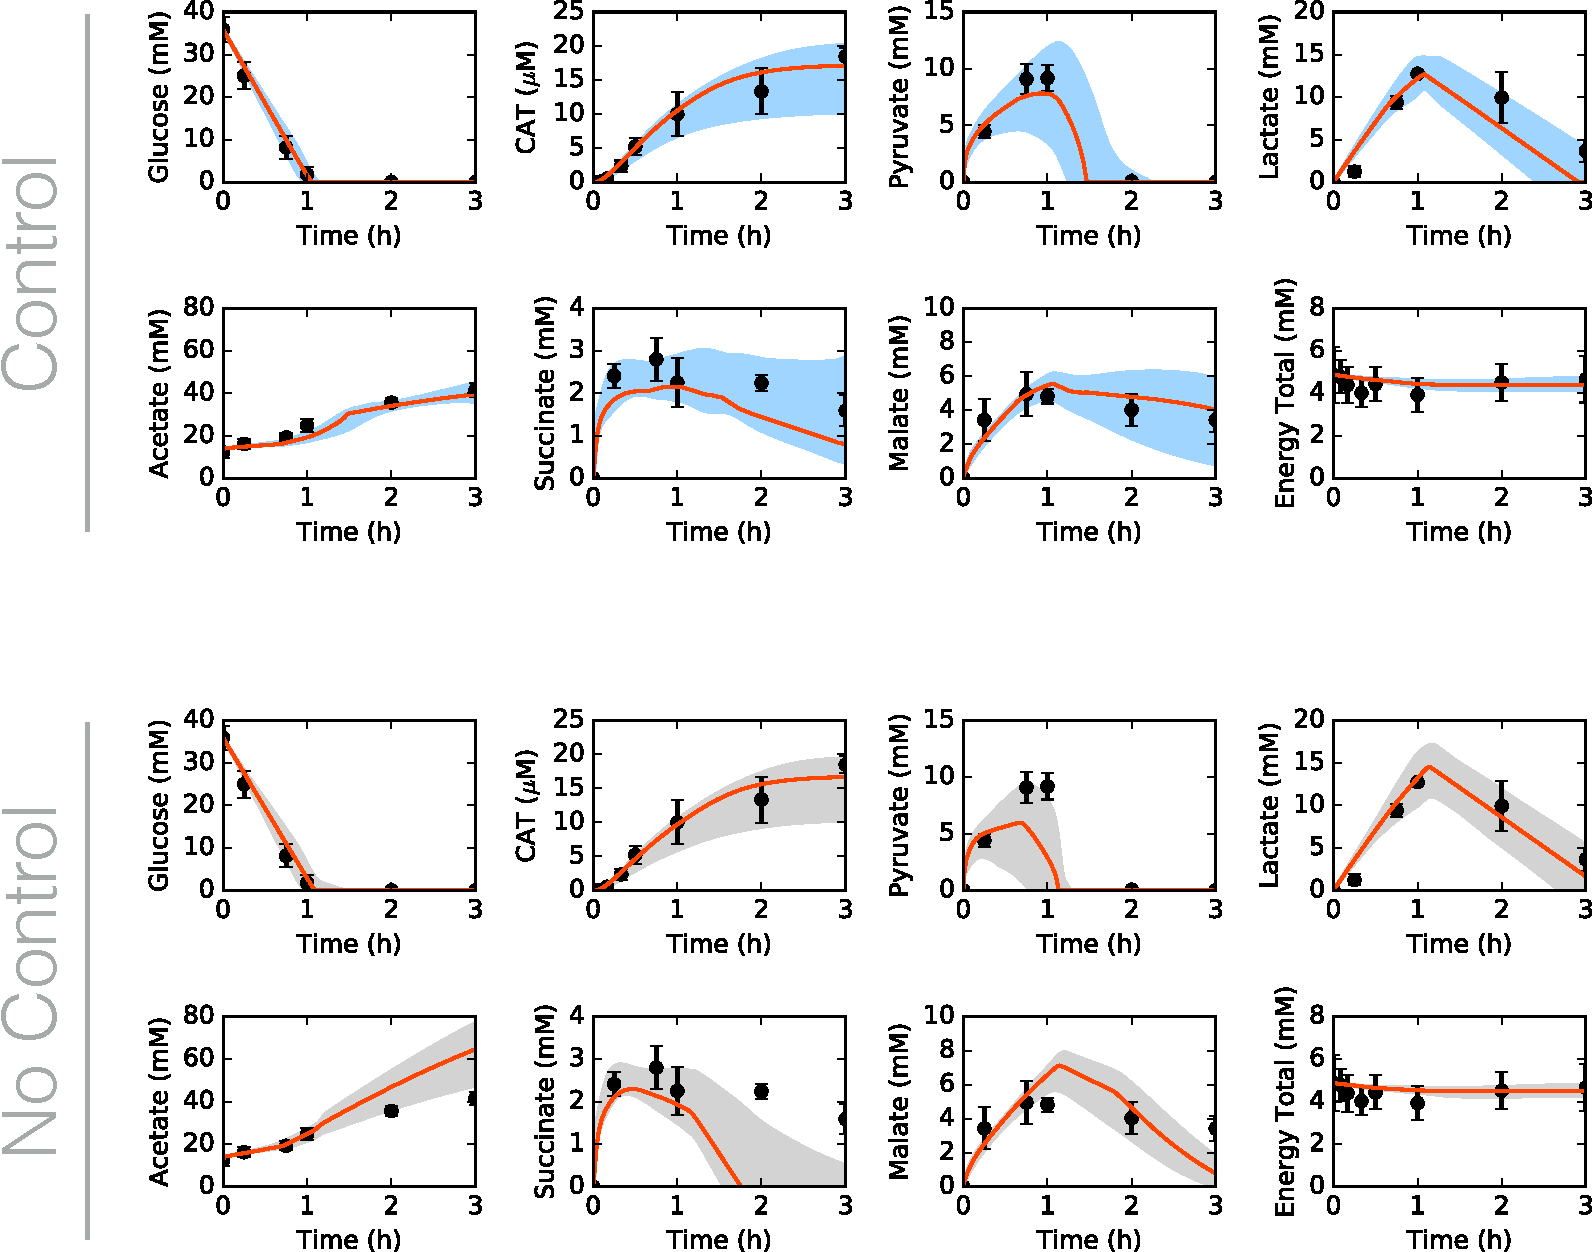
\includegraphics[width=1.00\textwidth]{./Figures/Fig_1_Carbon.pdf}
\caption{Central carbon metabolism in the presence (top) and absence (bottom) of allosteric control, including glucose (substrate), CAT (product), and intermediates, as well as total concentration of energy species. Best-fit parameter set (orange line) versus experimental data (points). 95\% confidence interval (blue or gray shaded region) over the ensemble of 100 sets.}
\label{fig:Carbon}
\end{figure}

\begin{figure}[ht]
\centering
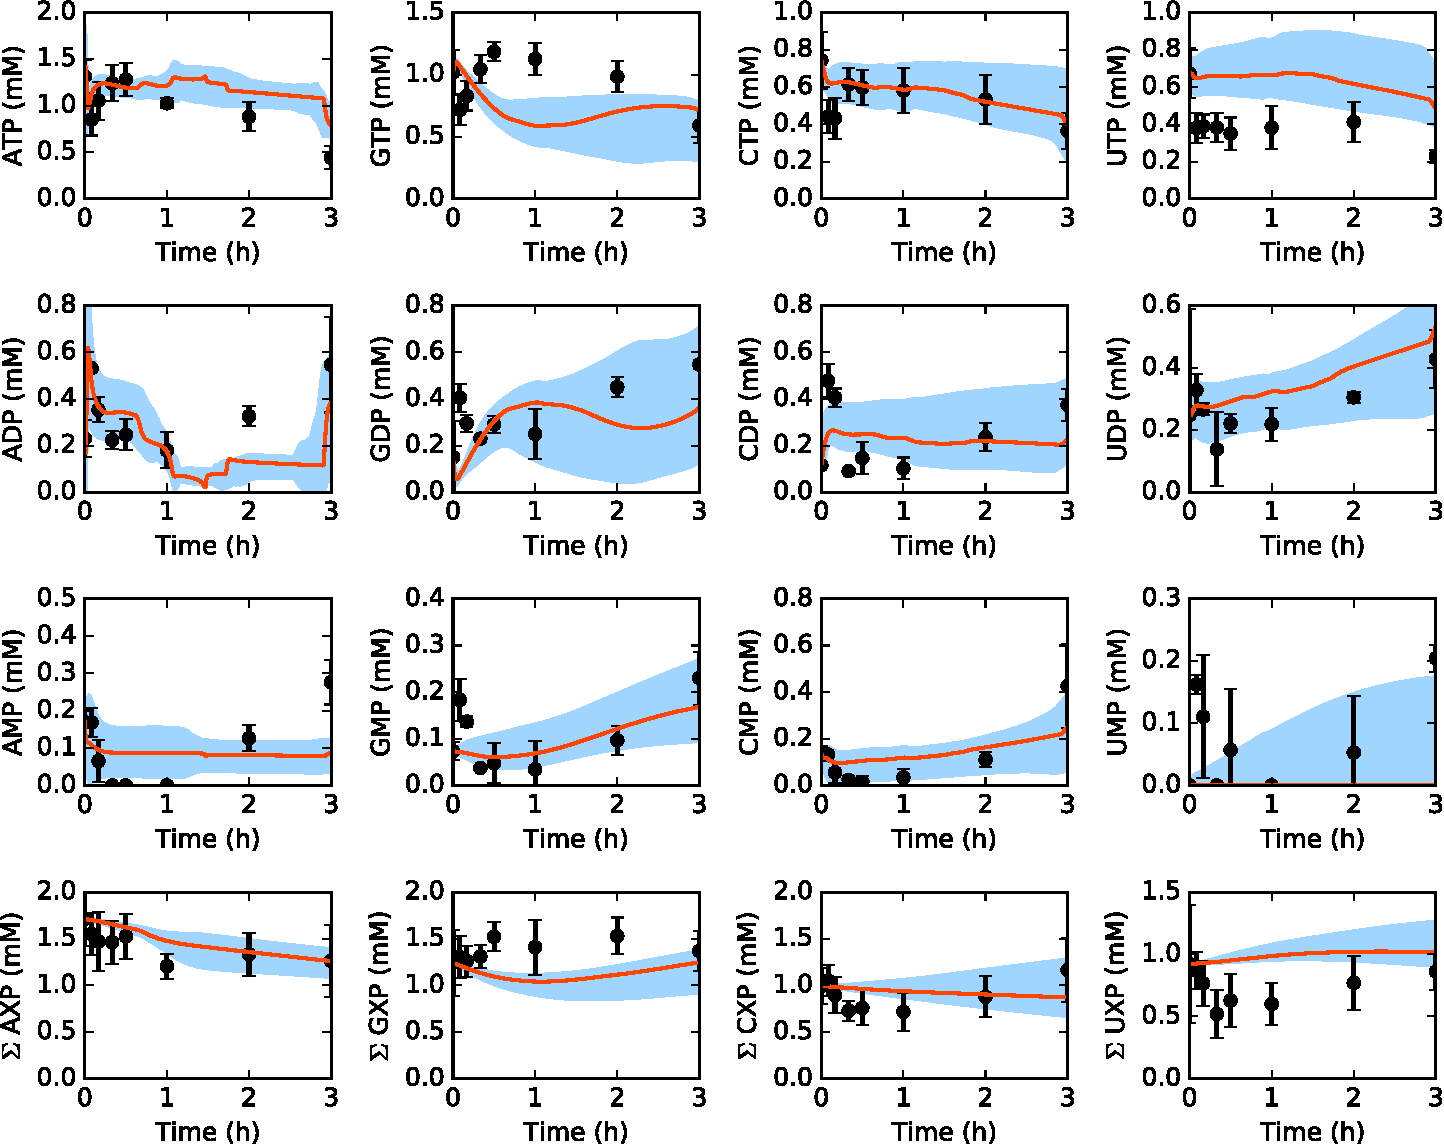
\includegraphics[width=1.00\textwidth]{./Figures/Fig_2_Energy.pdf}
\caption{Energy species and energy totals by base in the presence of allosteric control. Best-fit parameter set (orange line) versus experimental data (points). 95\% confidence interval (blue shaded region) over the ensemble of 100 sets.}
\label{fig:Energy}
\end{figure}

\begin{figure}[ht]
\centering
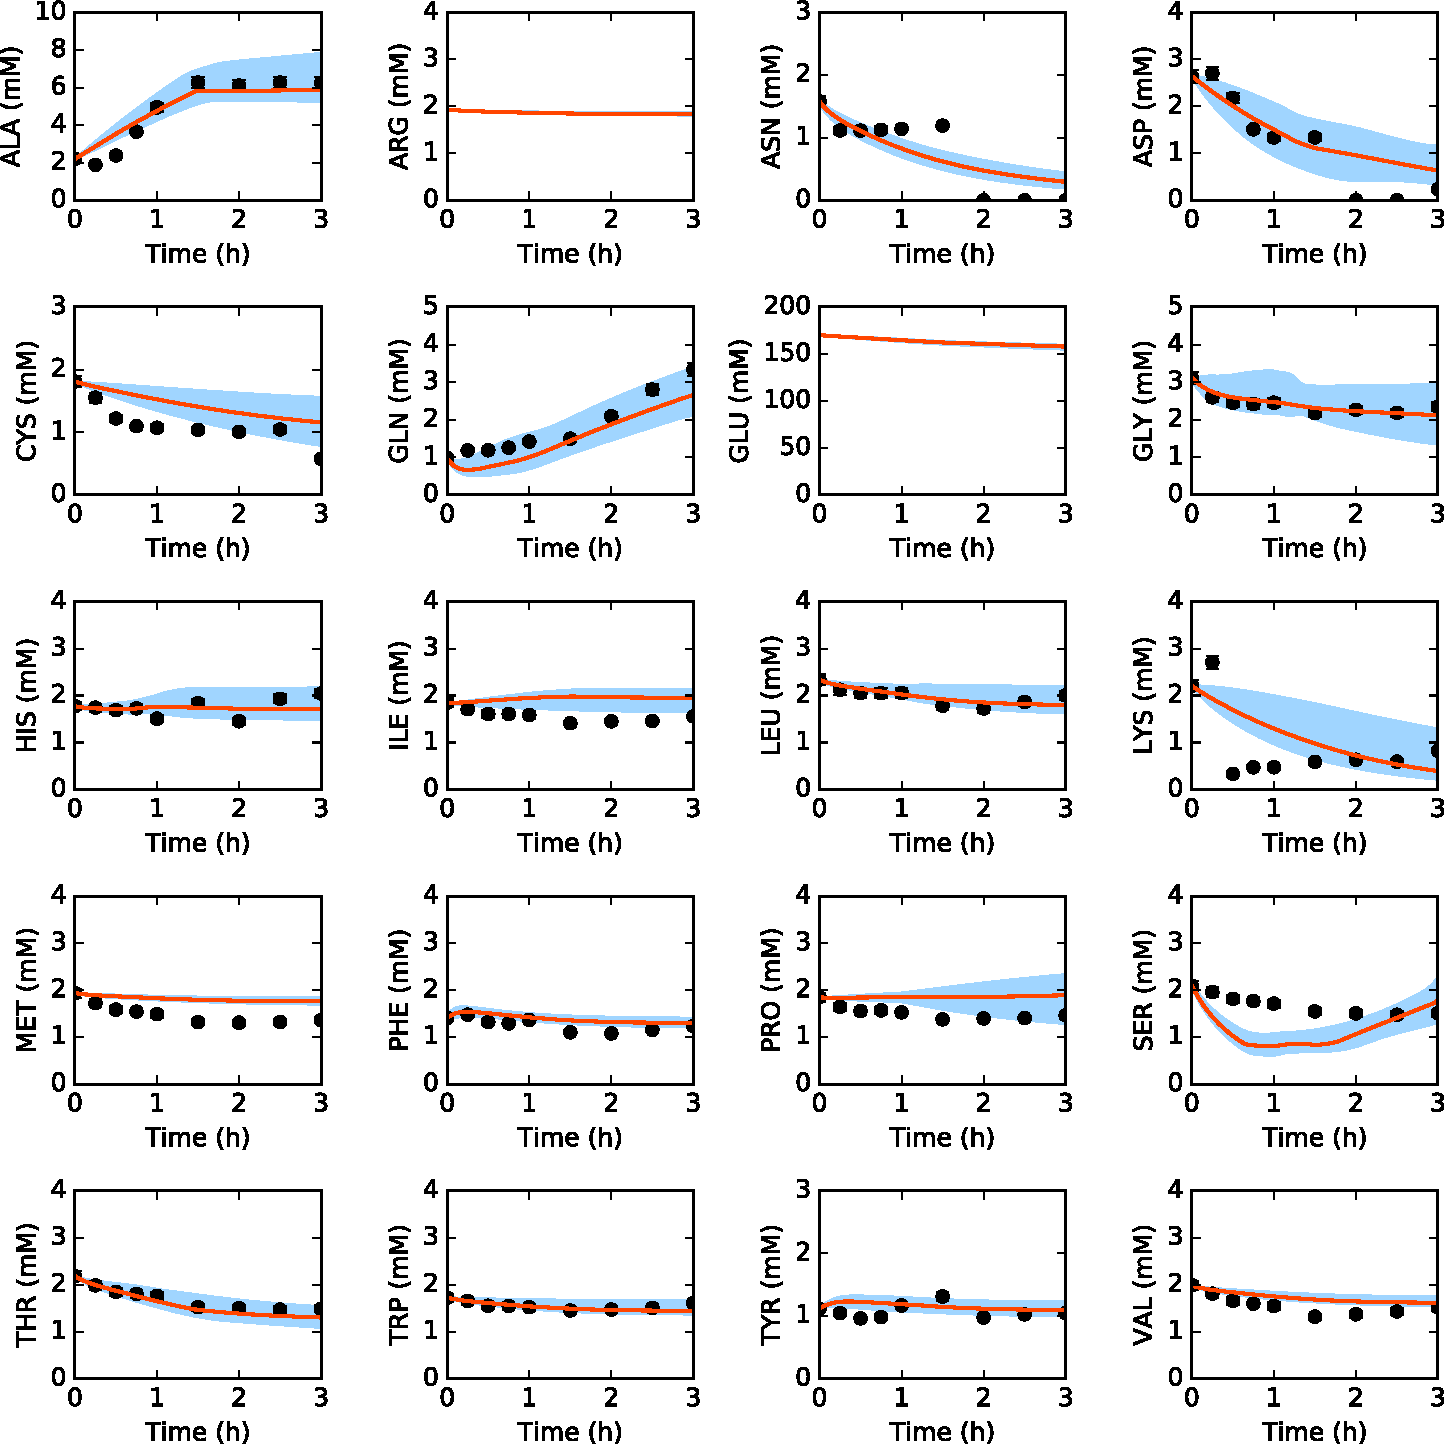
\includegraphics[width=1.00\textwidth]{./Figures/Fig_3_Amino.pdf}
\caption{Amino acids in the presence of allosteric control. Best-fit parameter set (orange line) versus experimental data (points). 95\% confidence interval (blue shaded region) over the ensemble of 100 sets.}
\label{fig:Amino}
\end{figure}

\begin{figure}[ht]
\centering
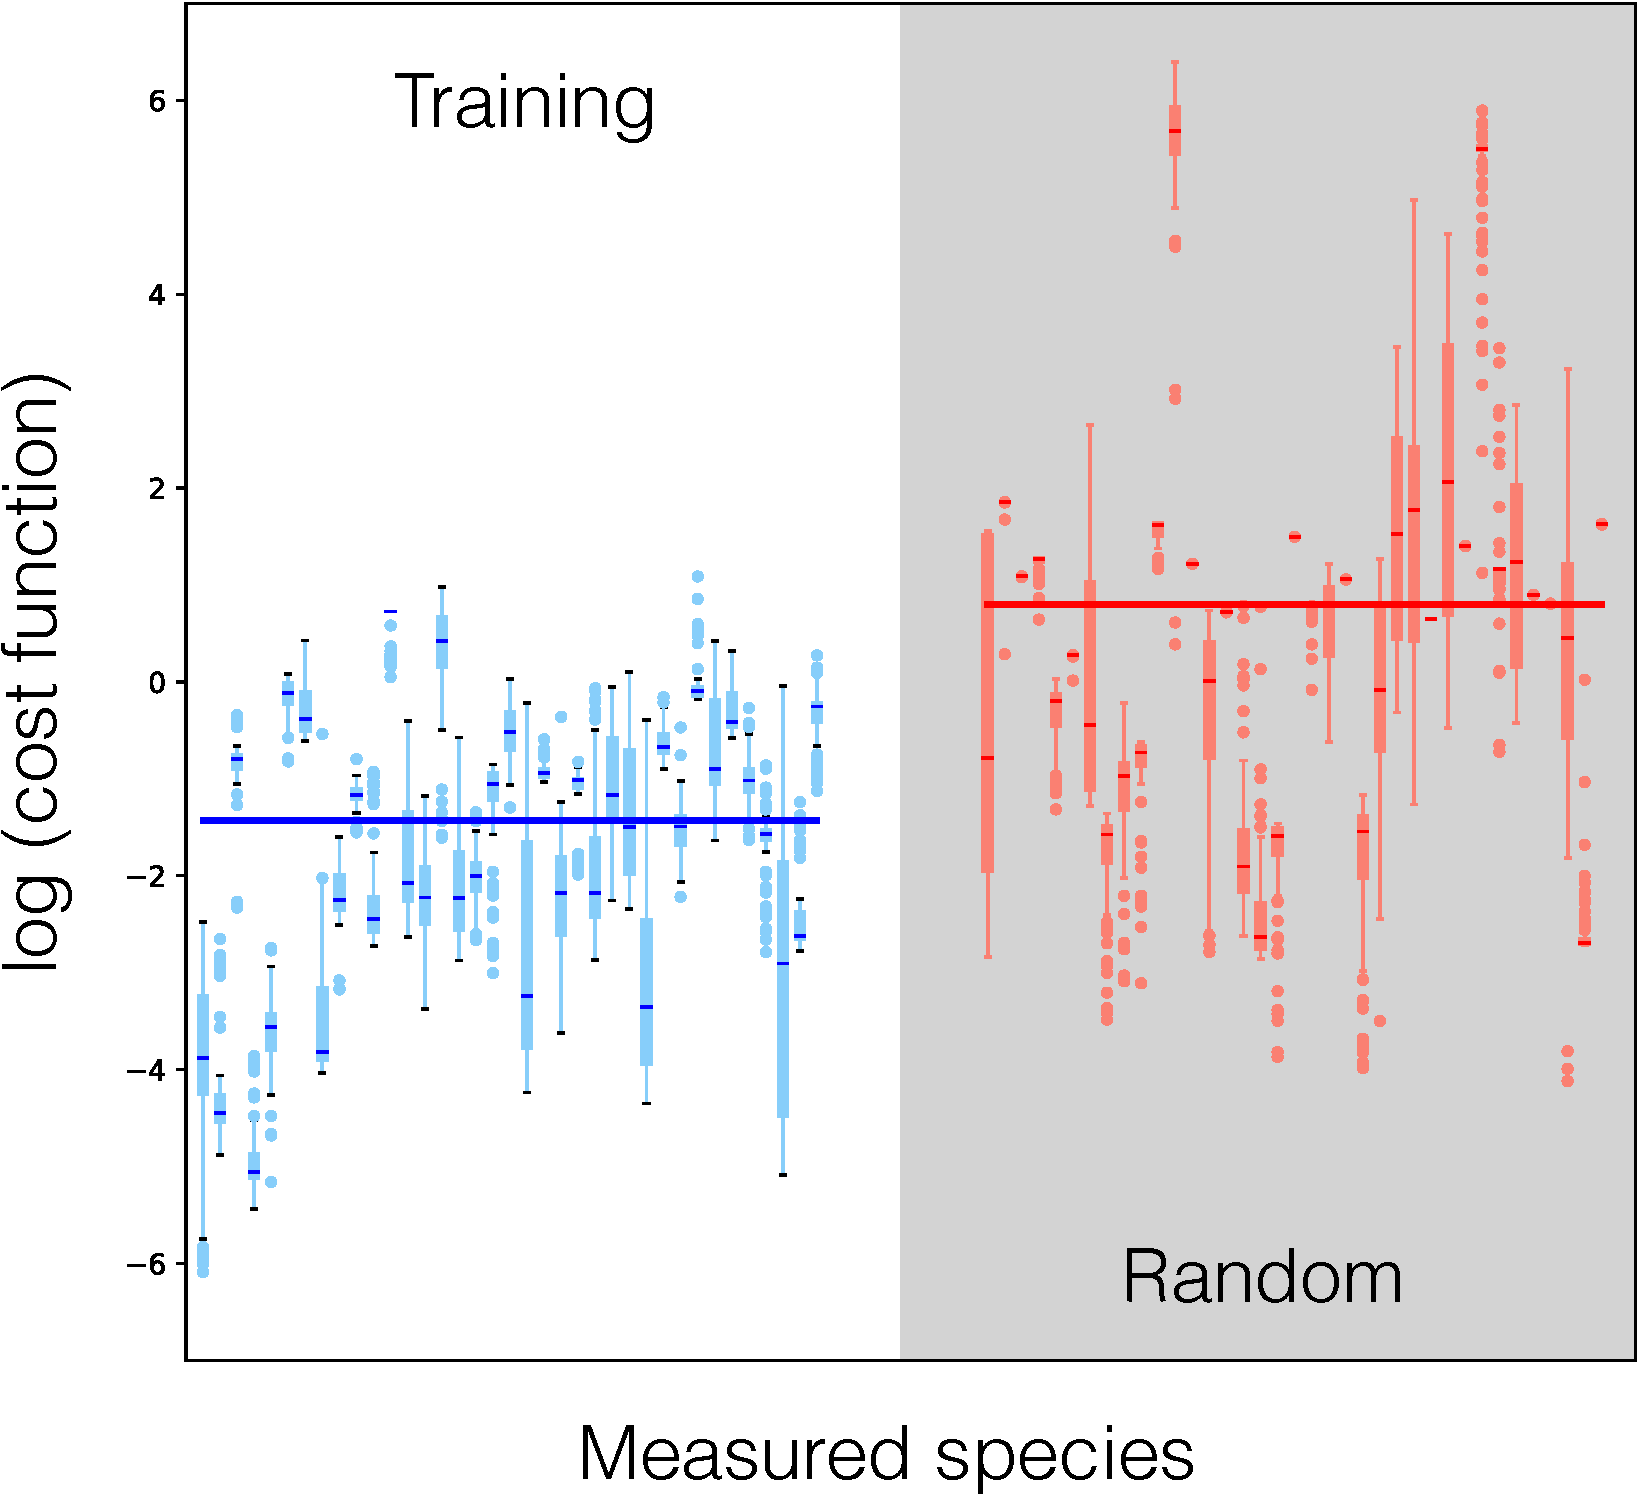
\includegraphics[width=1.00\textwidth]{./Figures/Fig_4_EnsembleVsRandom.pdf}
\caption{Log of cost function across 37 datasets for data-trained ensemble (blue) and randomly generated ensemble (red, gray background). Median (bars), interquartile range (boxes), range excluding outliers (dashed lines), and outliers (circles) for each dataset. Median across all datasets (large bar overlaid).}
\label{fig:BoxPlot}
\end{figure}

\begin{figure}[ht]
\centering
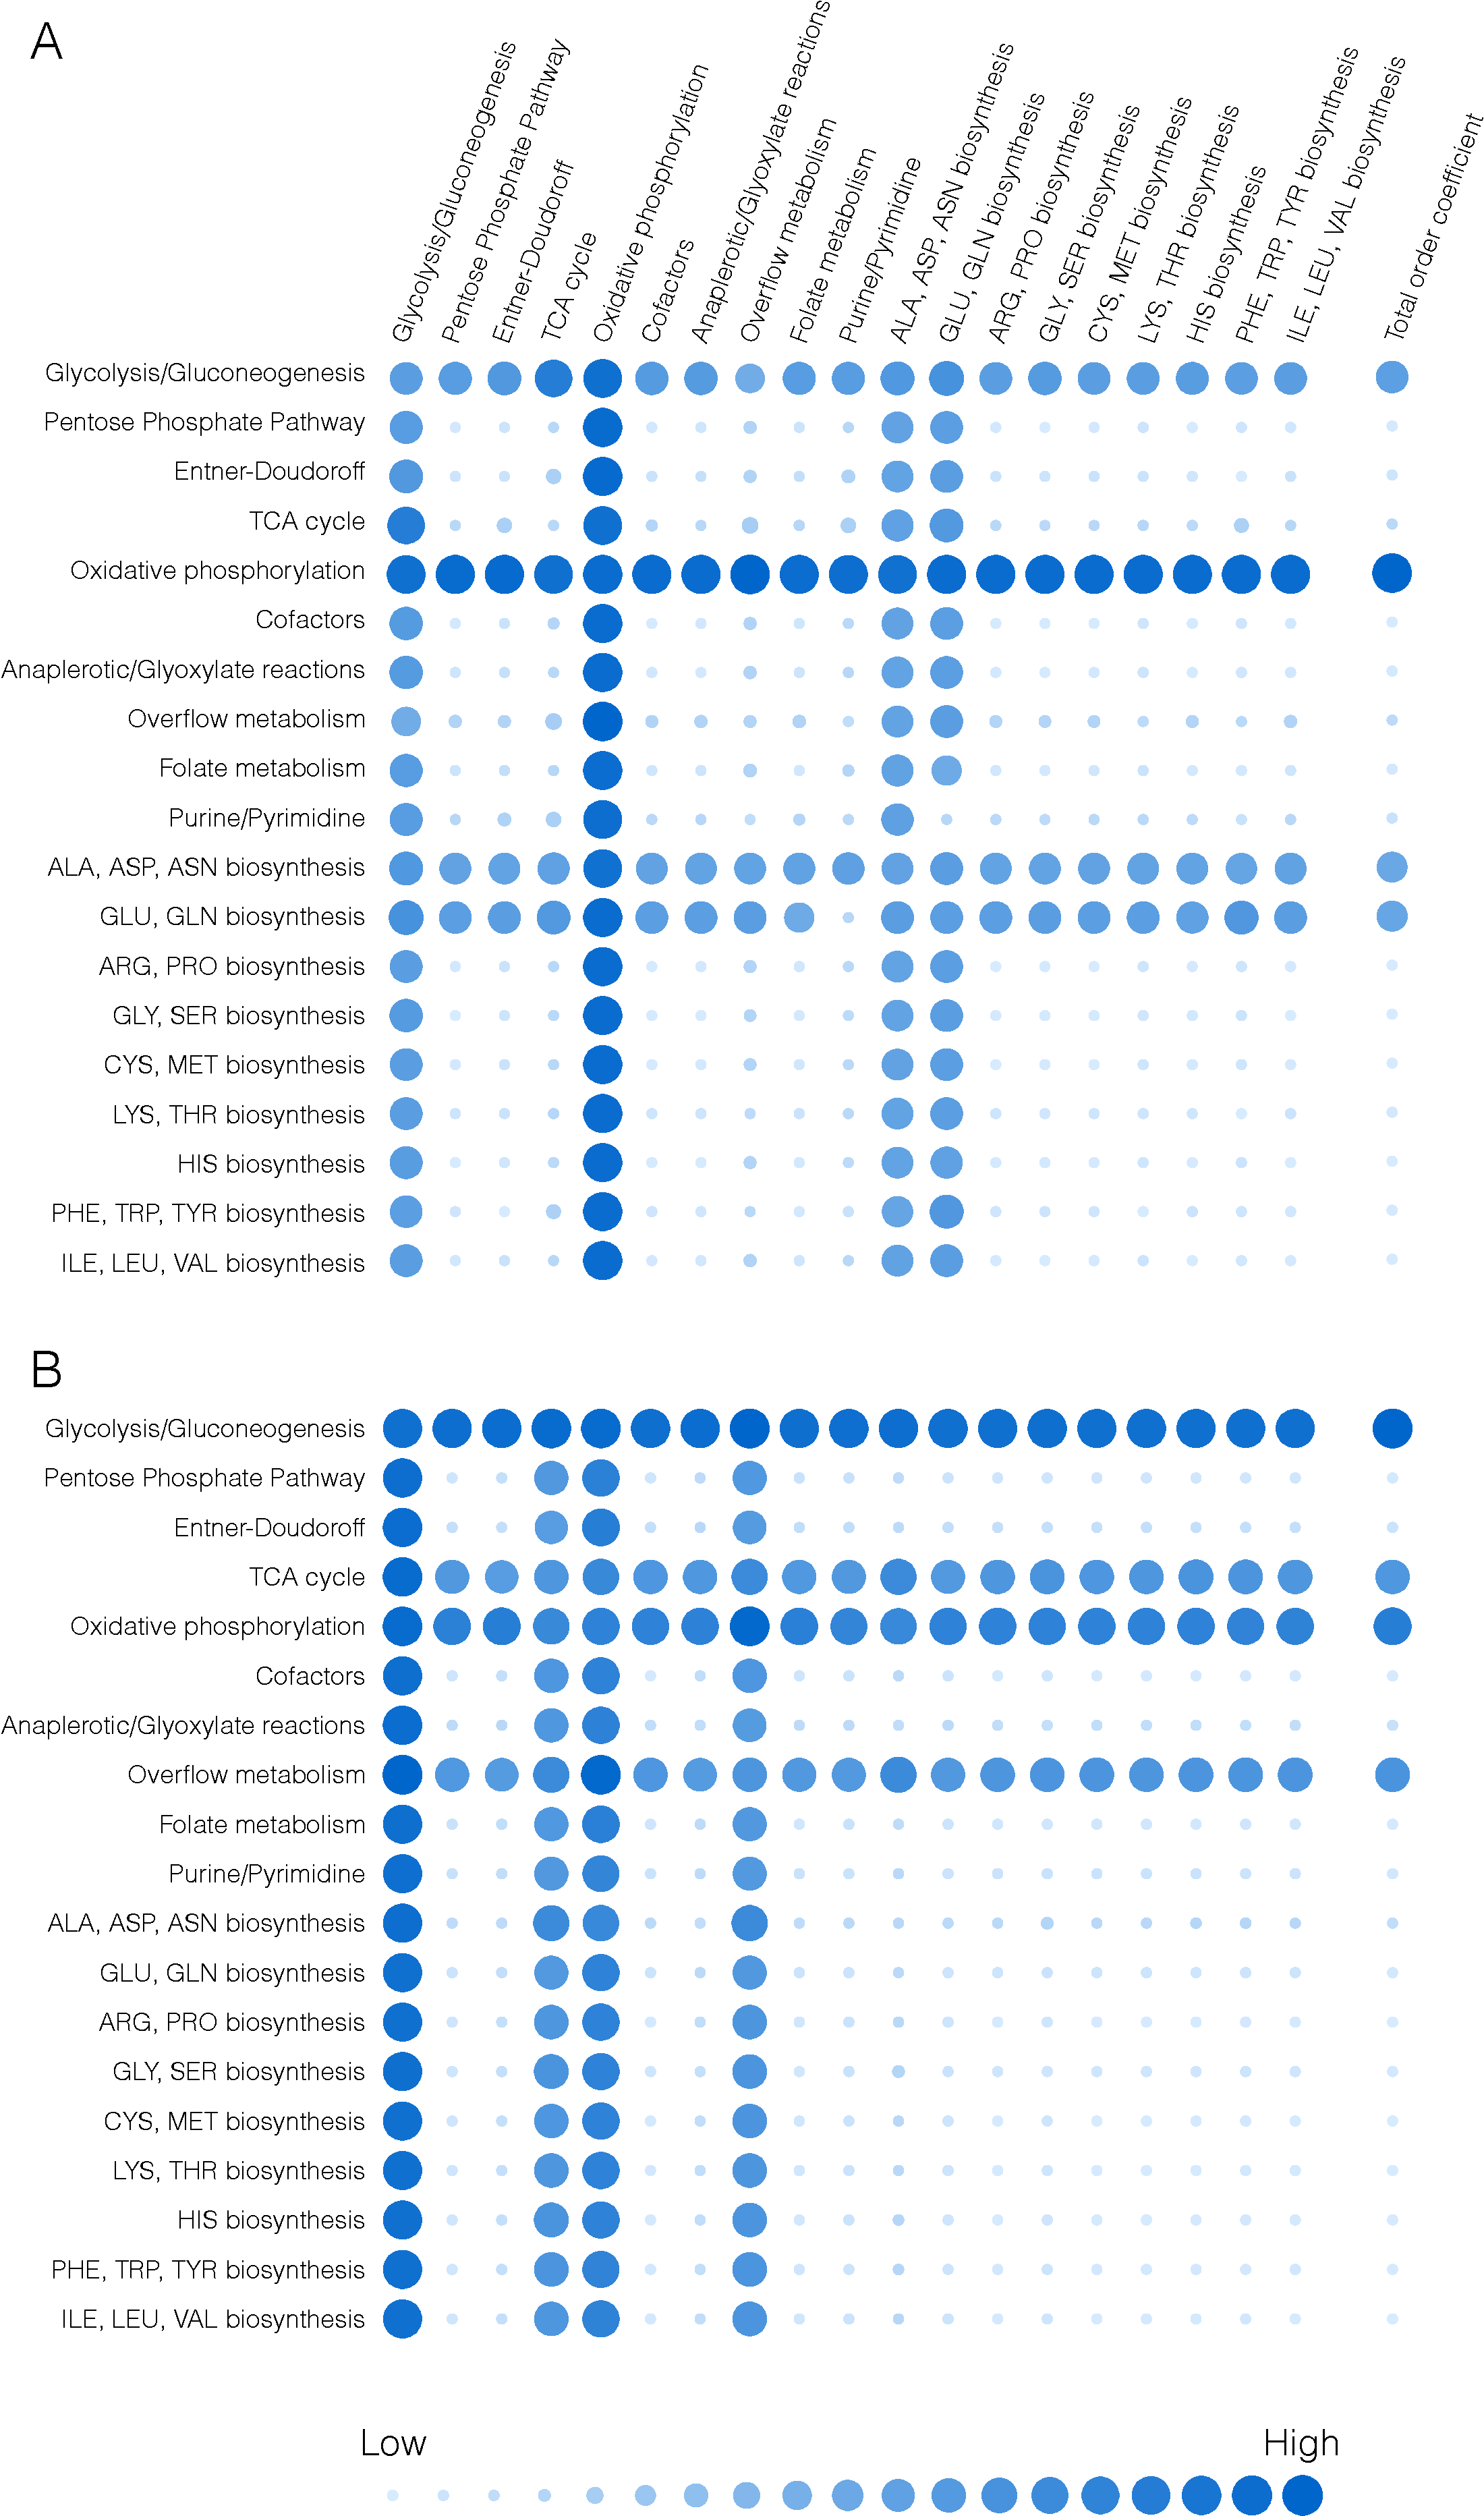
\includegraphics[width=0.7\textwidth]{./Figures/Fig_5_GroupKO.pdf}
\caption{Effect of group knockouts on system. A. Change in CAT productivity when one (diagonal) or two (off-diagonal) reaction groups are turned off. B. Change in system state (only species for which data exist) when one (diagonal) or two (off-diagonal) reaction groups are turned off. Total-order effect for each group calculated as the sum of first-order effect and all pairwise effects. Larger and darker circles represent greater effects.}
\label{fig:GroupKO}
\end{figure}

\clearpage

%\begin{table}
%\centering
% \caption{}
% \renewcommand{\arraystretch}{1.3}
% \begin{tabular}{llrrr} \toprule
% & \multicolumn{1}{r}{\textbf{Original value}} & \multicolumn{2}{r}{\textbf{After dilution factor}} & \textbf{BN ID} \\ \hline
%\smallskip
%\rule{0pt}{3ex} \parbox{4.3 cm}{Characteristic Enzyme Concentration} & \multicolumn{1}{r}{5 $\mu$M} & \multicolumn{2}{r}{0.1667 $\mu$M} & 100735 \\ \toprule
%\phantom{i}\textbf{Enzyme} & \textbf{Reaction name} & \textbf{Kcat (h$^-1$)} & 
% \textbf{Vmax (mM/h)} & \textbf{BN ID} \\ \hline
%\phantom{i}Serine dehydrase & R\_ser\_deg & 624000 & 104 & 101119 \\ \hline
%\phantom{i}Isocitrate dehydrogenase & R\_icd & 714000 & 119 & 101152 \\ \hline
%\phantom{i}Lactate dehydrogenase & R\_ldh & 348000 & 58 & 101036 \\ \hline
%\phantom{i}Aspartate transaminase & R\_aspC, R\_tyr, R\_phe & 1548000 & 258 & 101108 \\ \hline
%\phantom{i}Enolase & R\_eno & 792000 & 132 & 101028 \\ \hline
%\smallskip
%\rule{0pt}{3ex}
%Pyruvate kinase & R\_pyk & 1500000 & 250 & \parbox{1.4 cm}{101029, 101030} \\ \hline
%\phantom{i}Malic enzyme & R\_maeA, R\_maeB & 2124000 & 354 & 101167 \\ \hline
%\phantom{i}Phosphofructokinase & R\_pfk & 33264000 & 5544 & 104955 \\ \hline
%\phantom{i}Malate dehydrogenase & R\_mdh & 1980000 & 330 & 101163 \\ \hline
%\phantom{i}Citrate Synthase & R\_gltA & 2520000 & 420 & 101149 \\ \hline
%\phantom{i}6PG dehydrogenase & R\_zwf, R\_pgl, R\_gnd & 192000 & 32 & 101048 \\ \hline
%\phantom{i}Succinate dehydrogenase & R\_sdh & 7260 & 1.21 & 101162 \\ \hline
%\phantom{i}Succinyl-coA Synthetase & R\_sucCD & 282000 & 47 & 101158 \\ \hline
%\phantom{i}3PGA dehydrogenase & R\_gpm & 66000 & 11 & 101135 \\ \hline
%\phantom{i}PEP carboxylase & R\_ppc & 2124000 & 354 & 101139 \\ \hline
%\phantom{i}3PGA kinase & R\_pgk & 258000 & 43 & 101016 \\ \midrule
%\phantom{i}Geometric mean & & & 110 & \\ \toprule
%\phantom{i}\textbf{Transcription/Translation} & \textbf{AA-tRNA complex (mM)} & \textbf{Kcat (h$^-1$)} & \textbf{Vmax (mM/h)} & \textbf{BN ID} \\ \hline
%\phantom{i}tRNA charging & 0.03 & 14040 & 4212 & 104980 \\ \hline
%% Serine dehydrase & Yield & 8.1\% & 6.9\% & 2.6\% \\ \bottomrule
% \end{tabular}
%\label{tbl:Literature_values}
%\end{table}

\begin{table}
\centering
 \caption{}
 \renewcommand{\arraystretch}{1.3}
 \begin{tabular}{llrrr} \toprule
\smallskip
 & & \textbf{Original value} & \parbox{2.8 cm}{\textbf{After cell-free dilution factor}} & \textbf{BN ID} \\ \hline
\smallskip
\rule{0pt}{3ex} \parbox{4.3 cm}{Characteristic Enzyme Concentration} & & 5 $\mu$M & 167 nM & 100735 \\ \toprule
\phantom{i}\textbf{Enzyme} & \textbf{Reaction} & \textbf{Kcat (min$^{-1}$)} & 
 \textbf{Vmax (mM/h)} & \textbf{BN ID} \\ \hline
\phantom{i}Serine dehydrase & R\_ser\_deg & 10400 & 104 & 101119 \\ \hline
\phantom{i}Isocitrate dehydrogenase & R\_icd & 11900 & 119 & 101152 \\ \hline
\phantom{i}Lactate dehydrogenase & R\_ldh & 5800 & 58 & 101036 \\ \hline
\smallskip
\rule{0pt}{4.5ex}
Aspartate transaminase & \parbox{1 cm}{R\_aspC, R\_tyr, R\_phe} & 25800 & 258 & 101108 \\ \hline
\phantom{i}Enolase & R\_eno & 13200 & 132 & 101028 \\ \hline
\smallskip
\rule{0pt}{3ex}
Pyruvate kinase & R\_pyk & 25000 & 250 & \parbox{1.4 cm}{101029, 101030} \\ \hline
\smallskip
\rule{0pt}{3ex}
Malic enzyme & \parbox{1 cm}{R\_maeA, R\_maeB} & 35400 & 354 & 101167 \\ \hline
\phantom{i}Phosphofructokinase & R\_pfk & 554400 & 5544 & 104955 \\ \hline
\phantom{i}Malate dehydrogenase & R\_mdh & 33000 & 330 & 101163 \\ \hline
\phantom{i}Citrate Synthase & R\_gltA & 42000 & 420 & 101149 \\ \hline
\smallskip
\rule{0pt}{4.5ex}
6PG dehydrogenase & \parbox{1 cm}{R\_zwf, R\_pgl, R\_gnd} &3200 & 32 & 101048 \\ \hline
\phantom{i}Succinate dehydrogenase & R\_sdh & 121 & 1.21 & 101162 \\ \hline
\phantom{i}Succinyl-coA synthetase & R\_sucCD & 4700 & 47 & 101158 \\ \hline
\phantom{i}3PGA dehydrogenase & R\_gpm & 1100 & 11 & 101135 \\ \hline
\phantom{i}PEP carboxylase & R\_ppc & 35400 & 354 & 101139 \\ \hline
\phantom{i}3PGA kinase & R\_pgk & 4300 & 43 & 101016 \\ \midrule
\phantom{i}Geometric mean & & & 110 & \\ \toprule
\phantom{i}\textbf{Transcription/Translation} \\ \hline
%\phantom{i}\textbf{Transcription/Translation} & \textbf{AA-tRNA (mM)} & \textbf{Kcat (h$^-1$)} & \textbf{Vmax (mM/h)} & \textbf{BN ID} \\ \hline
\phantom{i}tRNA charging & 0.03 & 14040 & 4212 & 104980 \\ \hline
% \bottomrule
 \end{tabular}
\label{tbl:Literature_values}
\end{table}

%\begin{table}
%\centering
% \caption{}
% \renewcommand{\arraystretch}{1.3}
% \begin{tabular}{llrrr} \toprule
% & & \textbf{Original value} & \textbf{After dilution factor} & \textbf{BN ID} \\ \hline
%\smallskip
%\rule{0pt}{3ex} \parbox{4.3 cm}{Characteristic Enzyme Concentration} & & 5 $\mu$M & 0.1667 $\mu$M & 100735 \\ \toprule
%\phantom{i}\textbf{Enzyme} & \textbf{Reaction} & \textbf{Kcat (h$^-1$)} & 
% \textbf{Vmax (mM/h)} & \textbf{BN ID} \\ \hline
%\phantom{i}Serine dehydrase & R\_ser\_deg & 624000 & 104 & 101119 \\ \hline
%\phantom{i}Isocitrate dehydrogenase & R\_icd & 714000 & 119 & 101152 \\ \hline
%\phantom{i}Lactate dehydrogenase & R\_ldh & 348000 & 58 & 101036 \\ \hline
%\smallskip
%\rule{0pt}{4.5ex}
%Aspartate transaminase & \parbox{1 cm}{R\_aspC, R\_tyr, R\_phe} & 1548000 & 258 & 101108 \\ \hline
%\phantom{i}Enolase & R\_eno & 792000 & 132 & 101028 \\ \hline
%\smallskip
%\rule{0pt}{3ex}
%Pyruvate kinase & R\_pyk & 1500000 & 250 & \parbox{1.4 cm}{101029, 101030} \\ \hline
%\smallskip
%\rule{0pt}{3ex}
%Malic enzyme & \parbox{1 cm}{R\_maeA, R\_maeB} & 2124000 & 354 & 101167 \\ \hline
%\phantom{i}Phosphofructokinase & R\_pfk & 33264000 & 5544 & 104955 \\ \hline
%\phantom{i}Malate dehydrogenase & R\_mdh & 1980000 & 330 & 101163 \\ \hline
%\phantom{i}Citrate Synthase & R\_gltA & 2520000 & 420 & 101149 \\ \hline
%\smallskip
%\rule{0pt}{4.5ex}
%6PG dehydrogenase & \parbox{1 cm}{R\_zwf, R\_pgl, R\_gnd} & 192000 & 32 & 101048 \\ \hline
%\phantom{i}Succinate dehydrogenase & R\_sdh & 7260 & 1.21 & 101162 \\ \hline
%\phantom{i}Succinyl-coA synthetase & R\_sucCD & 282000 & 47 & 101158 \\ \hline
%\phantom{i}3PGA dehydrogenase & R\_gpm & 66000 & 11 & 101135 \\ \hline
%\phantom{i}PEP carboxylase & R\_ppc & 2124000 & 354 & 101139 \\ \hline
%\phantom{i}3PGA kinase & R\_pgk & 258000 & 43 & 101016 \\ \midrule
%\phantom{i}Geometric mean & & & 110 & \\ \toprule
%%\phantom{i}\textbf{Transcription/Translation} & \textbf{AA-tRNA (mM)} & \textbf{Kcat (h$^-1$)} & \textbf{Vmax (mM/h)} & \textbf{BN ID} \\ \hline
%\phantom{i}tRNA charging & 0.03 & 14040 & 4212 & 104980 \\ \hline
%% \bottomrule
% \end{tabular}
%\label{tbl:Literature_values}
%\end{table}

%\begin{table}
%\centering
%    \caption{CAT carbon yield breakdown for best-fit set, knockouts, and experimental data. Carbon produced as CAT, carbon consumed as glucose and each amino acid, sum of consumed species, and yield. Accumulation of alanine and glutamine (negative consumption terms) was not considered in yield calculation.}
%    \renewcommand{\arraystretch}{1.3}
%    \begin{tabular}{lrrrrrr} \toprule
%        Carbon Produced (C-mM) & Best-fit & $\Delta$app & $\Delta$nuo & $\Delta$cyd & \parbox{1 cm}{$\Delta$app $\Delta$nuo $\Delta$cyd} & Data \\ \hline
%        CAT & 20.9 & 21.4 & 18.1 & 6.5 & 5.1 & 21.6 \\ \midrule
%        Carbon Consumed (C-mM) \\ \hline
%        GLC & 215.4 & 215.4 & 215.4 & 215.4 & 159.8 & 215.4 \\ \hline
%        ALA & -11.6 & -11.4 & 1.7 & -3.8 & -3.2 & -12.1 \\ \hline
%%        ARG & 10.2 & 9.9 & 1.1 & 0.9 & 1.3 & - \\ \hline
%        ASN & 6.2 & 6.2 & 6.2 & 6.3 & 6.3 & 6.3 \\ \hline
%        ASP & 7.5 & 7.5 & 3.9 & 0.0 & 0.0 & 9.6 \\ \hline
%        CYS & 3.0 & 3.1 & 3.0 & 2.9 & 2.9 & 3.7 \\ \hline
%        GLN & -11.4 & -11.3 & -4.0 & 1.8 & 2.7 & -11.7 \\ \hline
%%        GLU & 492.6 & 505.6 & 528.2 & 505.1 & 501.8 & - \\ \hline
%        GLY & 3.1 & 3.1 & 2.6 & 1.1 & 0.9 & 1.5 \\ \hline
%        HIS & 0.2 & 0.2 & 1.1 & 0.4 & 0.3 & 0.0 \\ \hline
%        ILE & 1.0 & 1.0 & 0.8 & 0.3 & 0.2 & 1.7 \\ \hline
%        LEU & 1.4 & 1.4 & 1.2 & 0.4 & 0.3 & 2.0 \\ \hline
%        LYS & 10.7 & 10.7 & 13.1 & 13.2 & 13.2 & 8.3 \\ \hline
%        MET & 0.8 & 0.8 & 0.7 & 0.2 & 0.2 & 2.9 \\ \hline
%        PHE & 3.2 & 3.3 & 2.8 & 1.0 & 0.8 & 1.6 \\ \hline
%        PRO & 2.4 & 2.4 & 0.7 & 0.2 & 0.2 & 1.9 \\ \hline
%        SER & 2.5 & 2.5 & 2.4 & 2.1 & 2.1 & 1.8 \\ \hline
%        THR & 3.4 & 3.4 & 3.3 & 2.9 & 2.8 & 2.8 \\ \hline
%        TRP & 1.0 & 1.0 & 0.8 & 0.3 & 0.2 & 1.2 \\ \hline
%        TYR & 1.1 & 1.1 & 1.1 & 0.4 & 0.4 & 0.6 \\ \hline
%        VAL & 1.4 & 1.5 & 1.2 & 0.4 & 0.4 & 2.4 \\ \midrule
%%        Sum & 767.1 & 780.1 & 791.3 & 755.3 & 696.8 & - \\ \hline
%        Sum & 264.3 & 264.6 & 262.0 & 249.3 & 193.7 & 263.7 \\ \midrule
%%        Yield & 2.7\% & 2.7\% & 2.3\% & 0.9\% & 0.7\% & - \\ \hline
%        Yield & 7.9\% & 8.1\% & 6.9\% & 2.6\% & 2.7\% & 8.2\% \\ \bottomrule
%    \end{tabular}
%\label{tbl:yield_breakdown}
%\end{table}

\clearpage

\begin{figure}[ht]
\centering
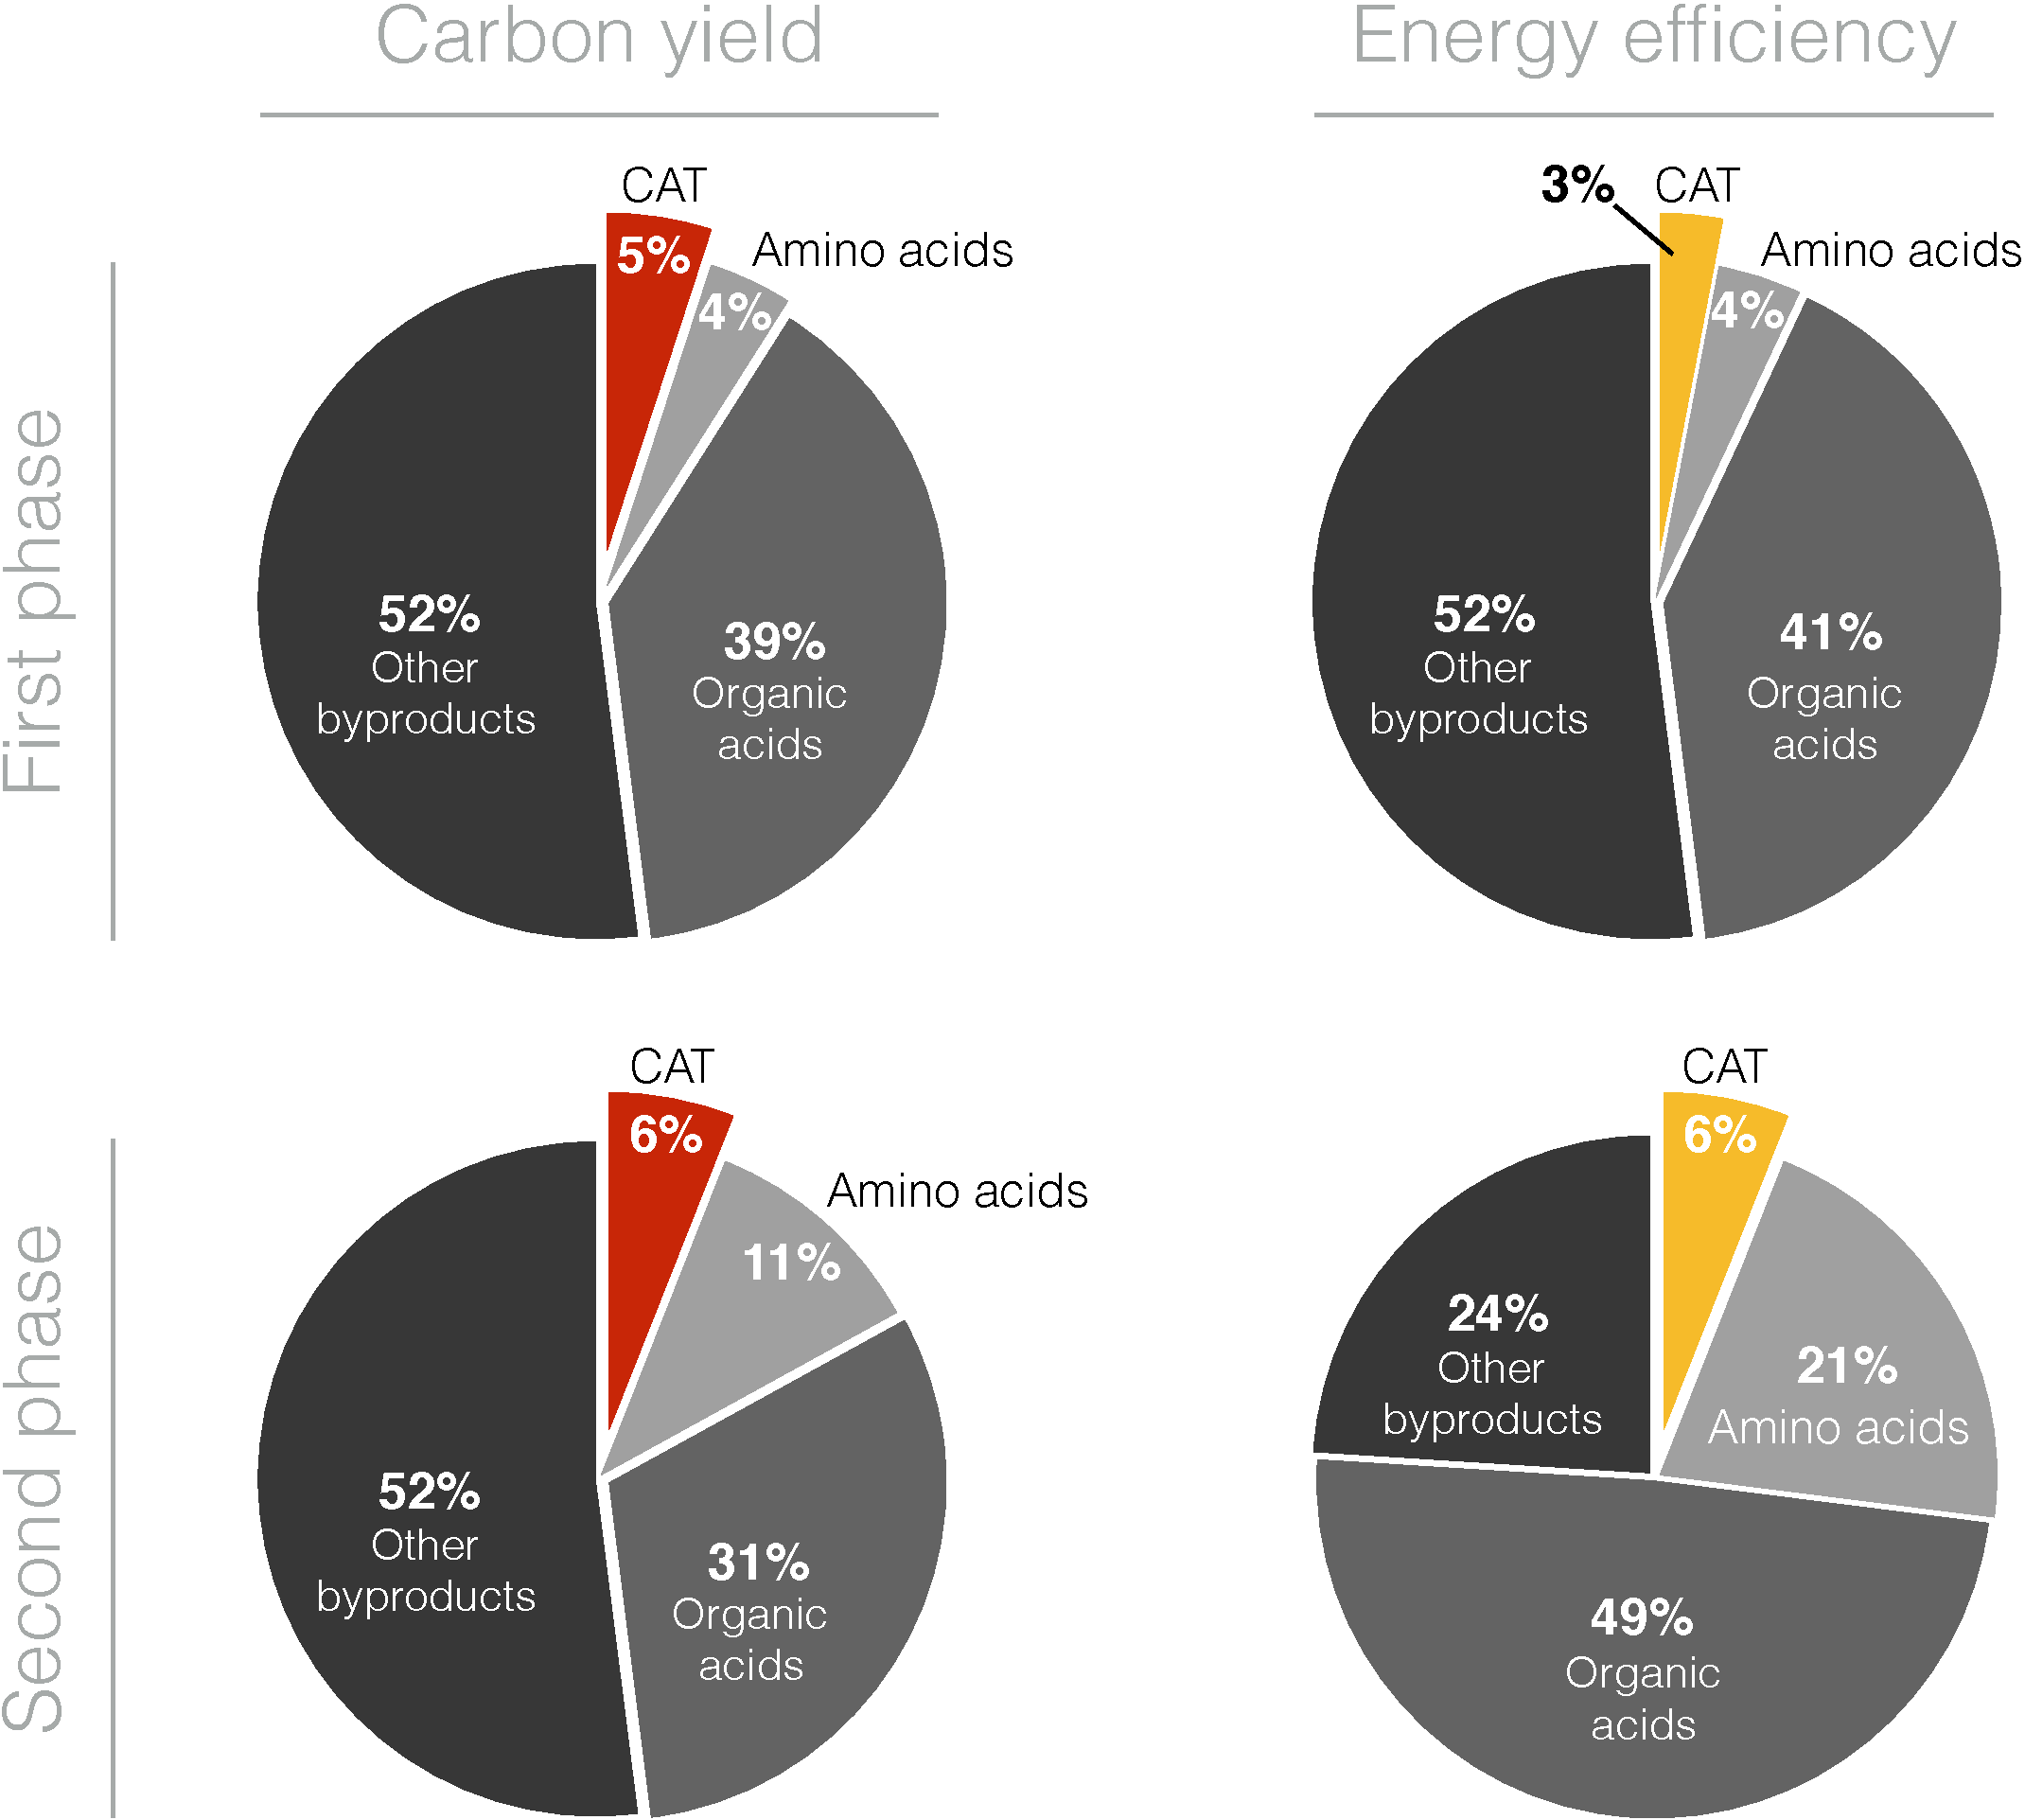
\includegraphics[width=0.6\textwidth]{./Figures/Fig_6_CarbonEnergyBalances.pdf}
%\caption{Carbon and energy balances for the best-fit set. A. Carbon moles produced as CAT, amino acids (alanine and glutamine), organic acids (lactate, acetate, succinate, and malate), and other byproducts including carbon dioxide, as percentages of total carbon consumption (glucose and all other amino acids). B. Energy cost of CAT production, accumulation of organic acids (lactate, acetate, succinate, and malate), and glycolytic and pentose phosphate metabolites, as percentages of total energy utilization from glucose. Energy costs calculated in terms of equivalent ATP molecules.}
\caption{Carbon and energy balances for the best-fit set. A. Carbon moles produced as CAT, amino acids (alanine and glutamine), organic acids (lactate, acetate, succinate, and malate), and other byproducts including carbon dioxide, as percentages of total carbon consumption (glucose and all other amino acids). B. Energy cost of CAT production, accumulation of amino acids (alanine and glutamine), accumulation of organic acids (lactate, acetate, succinate, and malate), and other byproducts, as percentages of total energy utilization from glucose. Energy costs calculated in terms of equivalent ATP molecules.}
\label{fig:CAT_balances}
\end{figure}

\clearpage

% Supplemental figures -
% Set the S-
\renewcommand\thefigure{S\arabic{figure}}
\renewcommand\thetable{T\arabic{table}}
\renewcommand\thepage{S-\arabic{page}}
\renewcommand\theequation{S\arabic{equation}}

% Reset the counters -
\setcounter{equation}{0}
\setcounter{table}{0}
\setcounter{figure}{0}
\setcounter{page}{1}

% Supplemental figures go here ...
%\begin{figure}[ht]
%\centering
%\includegraphics[width=1.00\textwidth]{./figs/<Filename>.pdf}
%\caption{Captiontext goes here}
%}\label{fig:<label_name>}
%\end{figure}

\end{document}
\grid
\grid
